\documentclass[conference]{IEEEtran}
\IEEEoverridecommandlockouts
% The preceding line is only needed to identify funding in the first footnote. If that is unneeded, please comment it out.
\usepackage{cite}
\usepackage{amsmath,amssymb,amsfonts}
\usepackage{algorithmic}
\usepackage{graphicx}
\usepackage[export]{adjustbox}
\usepackage{textcomp}
\usepackage{xcolor}
\usepackage[utf8]{inputenc}
\pagenumbering{roman}
\usepackage{longtable} % for 'longtable' environment
\usepackage{pdflscape} % for 'landscape' environment
\usepackage{tabularx,booktabs}
\newcolumntype{C}{>{\centering\arraybackslash}X} % centered version of "X" type
\setlength{\extrarowheight}{1pt}
\usepackage{lipsum}
\usepackage[utf8]{inputenc}
\usepackage[english]{babel}
\usepackage{fancyhdr}
\usepackage{lastpage}


\pagestyle{fancy}
\fancyhf{}

\rfoot{Page \thepage \hspace{1pt} of \pageref{LastPage}}
% \def\BibTeX{{\rm B\kern-.05em{\sc i\kern-.025em b}\kern-.08em
%     T\kern-.1667em\lower.7ex\hbox{E}\kern-.125emX}}
\begin{document}

\title{A Efficient Approach for Intrusion Detection in Sensor Networks\\
% {\footnotesize \textsuperscript{*}Note: Sub-titles are not captured in Xplore and
% should not be used}
% \thanks{Identify applicable funding agency here. If none, delete this.}
}

\author{\IEEEauthorblockN{ Sai Teja Gudupati}
\IEEEauthorblockA{\textit{Electrical and Computer Engineering} \\
\textit{University of Waterloo}\\
Waterloo, Canada \\
stgudipa@uwaterloo.ca}
\and
\IEEEauthorblockN{ Shadman Raihan}
\IEEEauthorblockA{\textit{Electrical and Computer Engineering} \\
\textit{University of Waterloo}\\
Waterloo, Canada \\
s2raihan@uwaterloo.ca}
\and
\IEEEauthorblockN{ Somesh Kumar Gupta}
\IEEEauthorblockA{\textit{Electrical and Computer Engineering} \\
\textit{University of Waterloo}\\
Waterloo, Canada \\
sk2gupta@uwaterloo.ca}
% \and
% \IEEEauthorblockN{4\textsuperscript{th} Given Name Surname}
% \IEEEauthorblockA{\textit{dept. name of organization (of Aff.)} \\
% \textit{name of organization (of Aff.)}\\
% City, Country \\
% email address or ORCID}
% \and
% \IEEEauthorblockN{5\textsuperscript{th} Given Name Surname}
% \IEEEauthorblockA{\textit{dept. name of organization (of Aff.)} \\
% \textit{name of organization (of Aff.)}\\
% City, Country \\
% email address or ORCID}
% \and
% \IEEEauthorblockN{6\textsuperscript{th} Given Name Surname}
% \IEEEauthorblockA{\textit{dept. name of organization (of Aff.)} \\
% \textit{name of organization (of Aff.)}\\
% City, Country \\
% email address or ORCID}
}

\maketitle

\begin{abstract}
Wireless sensor network (WSN) is revolutionizing the field of the Internet of Things (IoT) due to its ease of deployment along with real-time applications. The number of WSN devices connected to the Internet is increasing at a rapid rate and this connectivity is also leading to many Security vulnerabilities in the WSNs. Under such scenarios, it becomes critical to detect the correct type of Intrusion as early as possible to deploy corrective measures to minimize the risk. In this study, we choose an efficient algorithm from different Artificial Intelligence and Machine Learning algorithms (AI\&ML) for multi-class classification of different Denial of Service (DoS) Intrusions detection based on lowest Computational Complexity while considering the performance of the algorithm for multi-class classification as WSNs have limited resources allocated to it.    
\end{abstract}

\begin{IEEEkeywords}
DoS, WSNs, AI, ML\end{IEEEkeywords}

\section{Introduction}
Wireless sensor networks (WSNs) are one of the most emerging technologies due to its size, cost-effectiveness and easily deployable nature. Since WSNs is becoming a globally adopted technology, the privacy and security concerns of the network have become a key issue. Due to the self-configuring capabilities of WSN devices, it is vulnerable to various types of security attacks. This can lead to loss of control over the WSNs, security breach, eavesdropping and monetary loss. 

Denial of Service (DoS) is one of the most dangerous security attacks which denies an intended user by making the network resources temporarily unavailable. It does that by sending superfluous requests to overload the system. It uses a single connection to attack the server. DoS attacks can lead to a huge monetary loss for organizations and disrupt various services including healthcare, home, smart transport, smart tourism, smart energy etc \cite{li2011smart}. Researchers around the world have introduced various Intrusion detection systems (IDSs) to address this issue. IDS may use various detection techniques including anomaly, signature and specification whereas, in this paper, we mainly analyze anomaly-based IDS. The performance of the anomaly-based IDS depends on the classification algorithm and the dataset used for training the algorithm. The classification of various types of DoS attacks is done by analyzing network traffic logs which include information about both normal and abnormal cases. 

In this paper, the multi-class classification of various types of DoS attacks is performed using both Artificial Intelligence and Machine Learning (AI\&ML) algorithms. A total of 5 different AI and ML algorithms is chosen based on the Computational Complexity of the algorithm. Among the Machine Learning algorithms, Gaussian Naive Bayes, Random Forest and Decision Tree are selected as they have lower Computational Complexity as compared to other algorithms. Whereas in the case of Artificial Intelligence, Multilayer Perceptrons (MLPs) and Long Short Term Memory (LSTM) algorithms are selected as the MLPs can learn detailed features whereas LSTMs have better performance for sequential data. While applying these techniques for abnormality detection, the complexity of the algorithms and their performance for multi-class classification is taken into account while selecting the best algorithm for deploying in WSNs. Since most of the WSNs are placed in a remote area without a continuous power supply, the longevity of these networks becomes a vital issue. The approximate power consumption can be represented in terms of the complexity of the algorithms since it represents the number of resources that are required to run the algorithm. 

The KDD-CUP-99 \cite{KDDcup99} and NSL-KDD dataset \cite{NSL_kdd} are the two most common datasets used for the evaluation of signature-based IDS algorithms. KDD-CUP-99 has redundant data in the training set which makes the algorithms biased towards frequent records. Mahbod.et.al.~\cite{NSL_kdd} proposed NSL-KDD dataset which was immune to above-mentioned shortcomings of KDD-CUP-99 dataset \cite{KDDcup99}. Both KDD-CUP-99 and NSL-KDD dataset has 41 features and 23 attack types. The features of the dataset include various network parameters like duration, protocol type, service, flag etc. The dimensionality of the dataset is reduced by selecting 10 most important features out of 41 features by using the chi-squared algorithm \cite{chi2}. The number of samples for each of the attack types are different for both KDD-CUP-99 and NSL-KDD dataset. In KDD-CUP-99, smurf attack type has the highest number of samples in the dataset while the spy attack type has only 2 samples. On the other hand, the NSL-KDD dataset has the highest sample size for the benign attack type whereas the spy attack has the lowest sample size. Therefore, the dataset is not well balanced as it can be seen in the graph presented in Figure \ref{samples_kdd} and \ref{samples_nsl}. For implementing a multi-class classification a well-balanced dataset is required as each attack type should have a sufficient number of samples so that the algorithms can learn all the feature variations to effectively perform multi-class classification. KDD-CUP-99 and NSL-KDD dataset lack a sufficient number of samples for some of the attack types which affects the classification accuracy in some cases which is shown in the Results section. Due to the unbalanced dataset for different attack types, the performance of the Neural Networks(NNs) dropped while performing multi-class classification as NNs requires large dataset for training.  

%This issue is more severe in neural networks because the performance of a neural network generally increases with the increase of sample size. Hyperparameter tuning was done to improve the performance of the network while keeping the complexity of the algorithms as low as possible.\\
%WSN devices have various constraints in terms of processing power, memory, network bandwidth and power consumption. Generally, these types of devices are cheap to manufacture and use very weak processors with a small battery. So, reducing the complexity of the algorithm will increase the overall lifespan of the WSN devices while making it fast and responsive. In this paper, the Intrusion detection performance of each of the algorithms has been discussed and also a methodology was developed for choosing the best model while considering computational complexity. 

\section{Literature Review}
There are different studies \cite{verma2020machine}, \cite{NSL_kdd}, \cite{kim2020cnn},\cite{nagar2020novel}, \cite{su2020bat} and \cite{almseidin2019applying} conducted for DoS Intrusion Detection algorithms which is discussed in detail. The studies \cite{almseidin2019applying},\cite{verma2020machine},\cite{NSL_kdd},\cite{kim2020cnn} and \cite{su2020bat} has presented the problem of Intrusion Detection as binary classification problem and applied different AI\&ML algorithms for classification. However, this seems ineffective as in order to perform counter measures for the type of attack it is important to detect the type of DoS attack the network is being targeted with as the counter measures differ with the type of attack. Therefore, there is a need to perform multi-class classification to detect the type of DoS attack. There are studies \cite{kim2020cnn},\cite{su2020bat} that have conducted multi-class classification using different AI\&ML algorithms without considering the runtime complexity of the algorithms.    

%The Internet of Things (IoT) has seen massive growth in the last two decades. Since the number of connected devices is increasing rapidly, the reliability of the network has become a vital issue. Denial of Service (DoS) attack is regarded as one of the main threats in online services. DoS attacks system infrastructure by making the network resource unavailable to its intended users or flooding the targeted business’ network bandwidth. Intrusion Detection Systems (IDSs) analyze the computer network traffic logs to identify these malicious attacks.

KDD-CUP-99~\cite{KDDcup99} is one of the most used datasets for bench-marking IDSs. Mei.et.al~\cite{shyu2003novel} proposed a robust Principal Component Analysis(PCA) based classifier for intrusion detection. The classifier uses an unsupervised learning algorithm where anomalies are considered to be an outlier. This classifier has been applied on the KDD-CUP-99 dataset which has achieved 98.94\% in recall and 97.89\% in precision while keeping the false alarm rate at 0.92\% in case of binary classification. However, only a few IDS solutions are using anomaly detection approaches and experts think that this technology is not mature enough. 

The KDD-CUP-99 dataset lacks a well-balanced sample size for each of the attack types which is detrimental for multi-class classification. Mahbod.et.al.~\cite{NSL_kdd} pointed out this deficiency of the KDD-CUP-99 dataset and proposed a novel solution to fix it. The authors proposed NSL-KDD dataset which includes selected data from original KDD-CUP-99 dataset but immune to above-mentioned shortcomings.\\
Both KDD-CUP-99 and NSL-KDD dataset contains simulated attacks which falls one of the following four types.\\
\begin{enumerate}
    \item \textbf{Denial of Service Attack (DoS):} This type of attack is initiated by making computing resources busy which denies users from accessing a service.
    \item \textbf{User to Root Attack (U2R):} In this class of attack, the attacker gets the access of a legitimate account by sniffing password or social engineering. The attacker then uses the root access to exploit the vulnerability.
    \item \textbf{Remote to Local Attack (R2L):} This happens when the attacker uses some vulnerability to gain the local access of that machine. 
    \item \textbf{Probing Attack:} The attacker tries to gain information about the victim's computer network avoiding its security controls.
\end{enumerate}

The Original KDD dataset includes redundant samples in the training set which makes the classifier biased towards more frequent records. This bias prevents the algorithm from learning more harmful but infrequent records like User to Root Attack (U2R). The NSL-KDD dataset improves on the KDD-CUP-99 dataset by discarding redundant records and duplicate data in the training and testing sets accordingly. The new NSL-KDD data set is still vulnerable to some of the problems discussed by McHugh~\cite{mchugh2000testing}. However, it is still used as benchmarking data for various intrusion detection methods. 

The study by Jiyeon.et.al.\cite{kim2020cnn} proposes a Convolutional Neural Network (CNN) based system for detecting DoS attacks. The performance of the proposed CNN model was evaluated against a Recurrent Neural Network (RNN). Here, they have generated two different types of image datasets from the KDD-CUP-99 dataset. In the dataset, the grayscale set of images has one channel whereas the RGB images have 3 colour channels. For evaluation, 18 scenarios have been created considering various hyperparameters including image size, kernel size and the number of convolutional layers. In this study, both binary and multi-class classification is implemented however, for multi-class classification, they have considered only 3 types of DoS attacks. One possible reason for this kind of choice can be the small sample size of other types of attacks since the performance of CNN based algorithms increases with the increase of sample size. RGB images outperformed grayscale images in terms of accuracy in the case of both binary and multi-class classifications. It is also shown that the performance of the model increases when more than one convolutional layer is used for multi-class classification. Hyperparameter tuning was performed to find out the best possible model for the classification problem. Both CNN and RNN showed an accuracy of 99\% for binary classification. Whereas, for multi-class classification, CNN achieved an overall accuracy score of 99\% while RNN showed 100\%, 80\% and 85\% accuracy for Smurf detection, Neptune and Benign DoS attacks respectively.

Derhab.et.al \cite{weller2014survey} proposes an Anomaly-based detection mechanism for DoS attacks that have been classified into statistical and Machine Learning-based methods. In the Statistical method, the normal traffic profile is calculated using the mean and standard deviation of normal traffic. The benefit of the Statistical approach is lower detection time with a low computational cost. In Machine Learning methods, classification and ensemble learning algorithms have been used to learn the traffic.

The study by Amma.et.al\cite{amma2020statistical} is a Statistical method that uses the Class center-based triangle area vector (CCTAV) to calculate the class center of the dataset along with feature extraction. For each sample data, the triangle area vector (TAV) is generated. In this study, two different profiles are created one for the normal traffic and the other for the abnormal (attack) traffic. The normal traffic profile was created using the mean and standard deviation of Mahalanobis distance (MahD) by taking all normal traffic into account. By using this  Mahalanobis distance the traffic is predicted as normal or attack type. In addition, the study shows that CCTAV has a computational complexity of $O((e^2)^n)$ which is less as compared to the existing Statistical methods.

Nerijus.et.al \cite{paulauskas2017analysis} analyzed the effect of data pre-processing on detection accuracy with the NSL-KDD dataset. The study shows that data preprocessing plays a vital role in determining the precision and accuracy of a Machine Learning model. In addition, Suleman.et.al \cite{khan2018feature} found out some of the important features of the DoS attack by calculating the entropy and granulation in the dataset. In this approach, the weight of each feature was calculated using the entropy calculation and then the best features important for classifying the DoS attack types were presented. This method helps in reducing the dimension of the dataset.

Su.et.al.\cite{su2020bat} uses BLSTM (Bidirectional Long Short-term memory) and attention mechanism for intrusion detection. The key features for network traffic classification have been obtained by the attention mechanism which screens the network flow vector generated by the BLSTM model. They also employed multiple layers of the convolutional layer to extract the local features of traffic data for classification. The algorithm has five major components i.e input layer, multiple Layers, BSLTM layer, attention layer and output layer. This deep Neural Network doesn't require any feature extraction as it automatically extracts the key features of the dataset by using different layers. 

Subha.et.al\cite{subha2013survey} analyzed different Neural Network algorithms such as ART, ARTl, FUZZY ART, IVEBF and EBCS and pointed out their performance in improving the lifetime of a Wireless Sensor Networks (WSNs). The performance of a sensor network largely depends on the computational efficiency of the sensor node. Nowadays, a large number of smart sensor nodes are using Artificial Intelligence. So, it is of paramount importance that intelligent tools should be used in an energy-efficient way in the wireless sensor network. In addition, different types of Machine Learning techniques are introduced to reduce energy consumption along with a reduction in communication cost for WSNs. 

The study by Tao.et.al\cite{tao} uses a hybrid approach for detecting DoS Cyberthreats. The hybrid approach consists of ensemble learning in which the first step is to find clusters of different labels in the dataset using Spectral clustering. In the second step, it uses a Deep Neural Network(DNN) to do multi-class classification. It then predicts whether traffic is normal or whether an attack is being attempted by specifying which type of attack is being conducted on the network with an accuracy score. However, the hybrid approach mentioned by \cite{tao} uses unsupervised learning in the first step to cluster the labels which seems unreasonable as the DoS Cyber attacks are a Supervised learning problem. As given in \cite{spectral_clustering_CC} the Computational Complexity of Spectral Clustering algorithm is $\mathcal{O}(n^{3})$ which is very high. The clustering technique used increases the computational complexity with an increase in power consumption by the network. This, however, might not find large scale applications for detecting DoS Intrusions in WSNs as we know that power consumption in WSNs is a limited resource.  

Wireless sensor network has constraints in terms of processing power and energy consumption. A large network such as BLSTM and CNN is more resource-intensive and is not an ideal choice for intrusion detection such as DoS attacks in a Wireless Sensor Network. Our work aims to deploy efficient and low power consuming Machine Learning algorithms while improving intrusion detection performance in detecting different DoS Cyber attacks.

\section{Proposed System Design}
In order to find an efficient AI and ML Network to detect DoS attacks for Wireless Sensor Networks, it is important to consider parameters such as memory requirement, power consumption by the Network, Training Computation Complexity and Prediction Computation Complexity. 

For the DoS attack detection, we have shortlisted 3 Machine Learning Algorithms based on Computation Complexity for training and prediction and 2 Artificial Intelligence models based on the overall accuracy for a different type of DoS attack. 

\subsection{Computation Complexity}
Computational complexity or simply complexity of an algorithm is defined as the number of resources required to run a particular algorithm. Computational Complexity gives importance to time and memory requirements for an algorithm. As the amount of resources required to run an algorithm generally varies with the size of the input, the complexity is typically expressed as a function $n \rightarrow{} f(n)$, where $n$ is the size of the input and $f(n)$ is either the worst-case complexity (the maximum of the number of resources that are needed overall inputs of size $n$) or the average-case complexity (the average of the number of resources overall inputs of size $n$). Time complexity is generally expressed as the number of required elementary operations on an input of size $n$, where elementary operations are assumed to take a constant amount of time on a given computer and change only by a constant factor when running on a different computer. Space complexity is generally expressed as the amount of memory required by an algorithm on an input of size $n$. 

After an analysis, we have come up with 3 Machine Learning algorithms that will be efficient for DoS attack detection. The algorithms are given below in Table \ref{tab1: Table 1} as per their Training Complexity and Prediction Complexity.


\begin{table}[h]
\centering
\caption{Computational Complexity of Machine Learning Algorithms}
\label{tab1: Table 1}
\begin{IEEEeqnarraybox}[\IEEEeqnarraystrutmode\IEEEeqnarraystrutsizeadd{2pt}{1pt}]{v/c/v/r/v/c/v}
\IEEEeqnarrayrulerow\\
& \mbox{{\bf Algorithms}} && \mbox{{\bf Training Complexity}} && \mbox{{\bf Prediction Complexity}} &\\
\IEEEeqnarraydblrulerow\\
\IEEEeqnarrayseprow[3pt]\\
& \mbox{Random Forest } && \mbox{$\mathcal{O}(n^{2}\ f\ n_{trees})$} && \mbox{$\mathcal{O}(f\ n_{trees})$} &\IEEEeqnarraystrutsize{0pt}{0pt}\\
\IEEEeqnarrayseprow[3pt]\\
\IEEEeqnarrayrulerow\\
\IEEEeqnarrayseprow[3pt]\\
& \mbox{Decision Tree} && \mbox{$\mathcal{O}(n^{2}\ f)$} && \mbox{$\mathcal{O}(f)$} &\IEEEeqnarraystrutsize{0pt}{0pt}\\
\IEEEeqnarrayseprow[3pt]\\
\IEEEeqnarrayrulerow\\
\IEEEeqnarrayseprow[3pt]\\
& \mbox{Naive Bayes} && \mbox{$\mathcal{O}(n\ f)$} && \mbox{$\mathcal{O}(f)$} &\IEEEeqnarraystrutsize{0pt}{0pt}\\
\IEEEeqnarrayseprow[3pt]\\
\IEEEeqnarrayrulerow\\
\IEEEeqnarrayseprow[3pt]\\
\IEEEeqnarrayseprow[0.5pt]\\
\IEEEeqnarrayrulerow
\end{IEEEeqnarraybox}
\end{table}

In Table \ref{tab1: Table 1}, $n$ is the number of training samples in the training dataset and $f$ is the number of features in the dataset whereas $n_{trees} $ is the depth of the tree or the number of trees depending on the implementation of the Random Forest algorithm.

From Table \ref{tab1: Table 1}, it is clear that the Naive Bayes algorithm will be more efficient than that of the Decision Tree algorithm when we consider both Training and Prediction Complexity. However, the two algorithms have the same Prediction Computation Complexity. Random Forest algorithm has higher Training and Prediction Complexity when compared to both Naive Bayes and Decision Tree by a factor of $n_{trees} $. Therefore, the decision to efficiently design the network for DoS Cyberthreat detection using Machine Learning algorithms depends entirely on the prediction accuracy of the Naive Bayes and Decision Tree algorithm. The higher the prediction accuracy for the dataset that particular algorithm will be chosen for the network design.

\begin{table}[h]
\centering
\caption{Computational Complexity of Neural Networks}
\label{tab1: Table 2}
\begin{IEEEeqnarraybox}[\IEEEeqnarraystrutmode\IEEEeqnarraystrutsizeadd{2pt}{1pt}]{v/c/v/r/v/}
\IEEEeqnarrayrulerow\\
& \mbox{{\bf Algorithms}} && \mbox{{\bf Prediction Complexity}} &\\ 
\IEEEeqnarraydblrulerow\\
\IEEEeqnarrayseprow[3pt]\\
& \mbox{Neural Network} && \mbox{$\mathcal{O}(f n_{l_{1}} + n_{l_{1}} n_{l_{2}} + ...)$} &\IEEEeqnarraystrutsize{0pt}{0pt}\\
\IEEEeqnarrayseprow[3pt]\\
\IEEEeqnarrayseprow[3pt]\\
\IEEEeqnarrayrulerow\\
\IEEEeqnarrayseprow[3pt]\\
\IEEEeqnarrayseprow[0.5pt]\\
\IEEEeqnarrayrulerow
\end{IEEEeqnarraybox}
\end{table}

In Table \ref{tab1: Table 2}, $f$ is the number of features in the dataset whereas, $n_{l_{i}}$ is the number of neurons at layer $i$ in a neural network. 
For DoS attack detection Multilayer Perceptrons (MLP) and LSTM (Long Short Term Memory) Recurrent Neural Network are considered due to their large applicability in different domains. 

As of now in choosing the most efficient model for DoS Cyber threat detection is incomplete as the analysis on Power Consumption is not completed for all the models. Once, when we calculate the power consumption on all the models for the given dataset then an overall comparison for selecting the most efficient algorithm for different DoS Cyberthreats Detection.  

\section{Metrics}
There are three metrics used for evaluating the models they are as given below: 

\subsection{Accuracy Score}
Accuracy is defined as the closeness of measurement to a particular value. Accuracy is used when the different classes in the dataset are well balanced. Accuracy Score is given by the formula below: 

\begin{equation}
    Accuracy = \frac{TP + TN}{TP + FP + TN + FN} 
    \label{eq:02}
\end{equation}

Where TP is True Positive, TN is True Negative, FP is False Positive and FN is False Negative.

\subsection{F1-Score}
F1-Score, also known as F-Score or F-Measure is a measure of a Test's accuracy. F1-score takes the harmonic mean of the precision and recall. It computes the result by the given formula below: 
\begin{equation}
    F1\ Score = 2 * \frac{Precision * Recall}{Precision + Recall}
    \label{eq:01}
\end{equation}

F1-Score is mainly used when the classes in the dataset are unbalanced. The maximum value attained by F1-score is 1 and it is also know as the Dice similarity coefficient.

\subsection{RoC Curve}
The Receiver Operating Characteristic curve (RoC) is a useful tool to find models for classification based on their performance by considering the False Positive Rate (FPR) and True Positive Rate(TPR). These values are computed by shifting the decision threshold of the classifier. On the RoC curve the TPR feature on the Y-axis whereas, FPR feature on the X-axis. Therefore the ideal point for the classifier is at the top left corner where the FPR is zero and TPR is 1 making the classifier ideal for the problem. The larger the area under the curve the better the performance of the classifier.     

\section{Experimental Results}

In this section, we discuss the results obtained from each algorithm. The main metrics used for evaluating the algorithms are F1-score, Accuracy Score and RoC curve and analysis is laid out for each of the algorithms as per the dataset. The tables \ref{tab1: Table 3} and \ref{tab1: Table 4} below shows the average accuracy for each of the dataset. Here for the entire dataset, the target accuracy is computed for Multi-class classification.  

The Figure \ref{samples_kdd} below shows the number of samples in KDD-CUP-99 \cite{KDDcup99} dataset. As from the Figure \ref{samples_kdd}, it is clear that the dataset is not balanced as few attack types have less than 100 samples whereas others have more than 1000 samples. This unbalanced dataset can affect the performance of the algorithms.  

\begin{figure}[h]
% 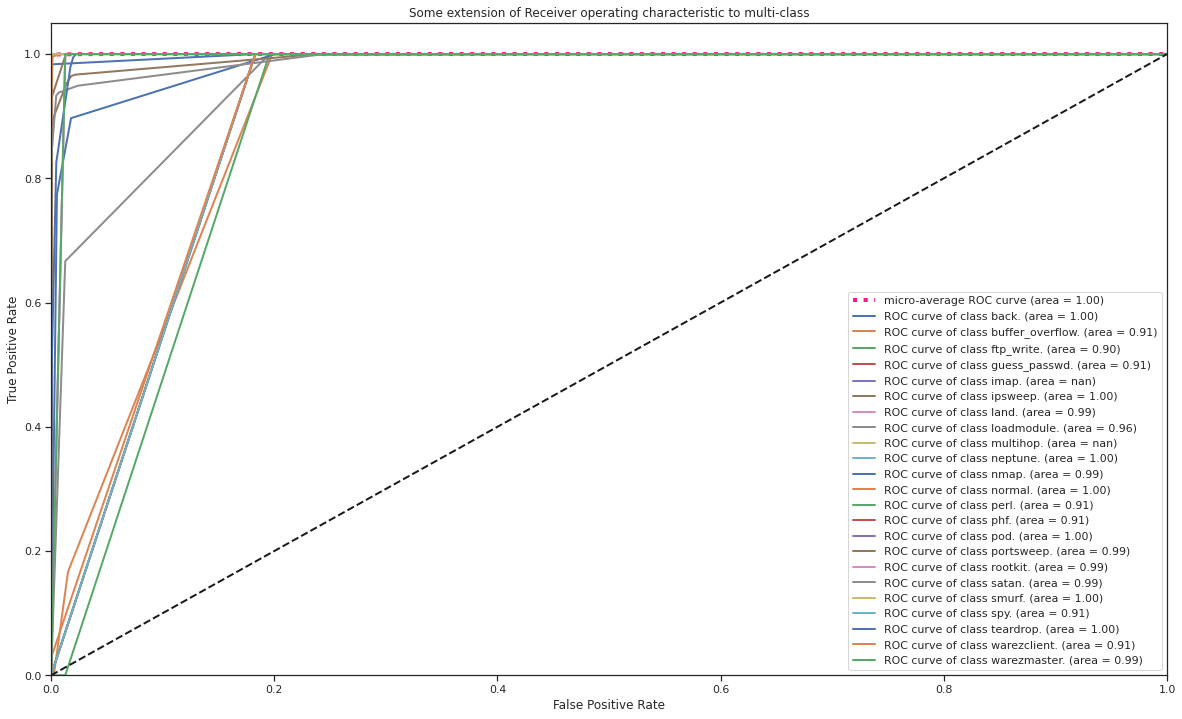
\includegraphics[max size={\textwidth}{\textheight}, angle = 90]{DT_KDD.png}
% \centerline{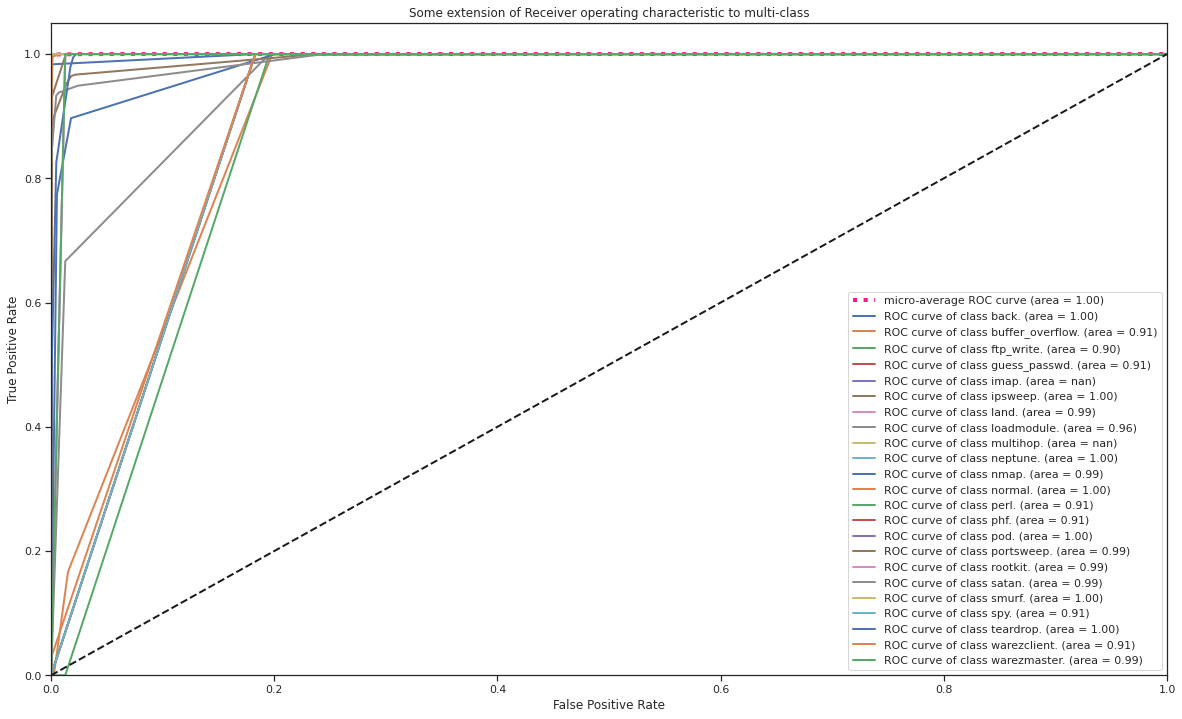
\includegraphics[width=8cm]{DT_KDD.png}}
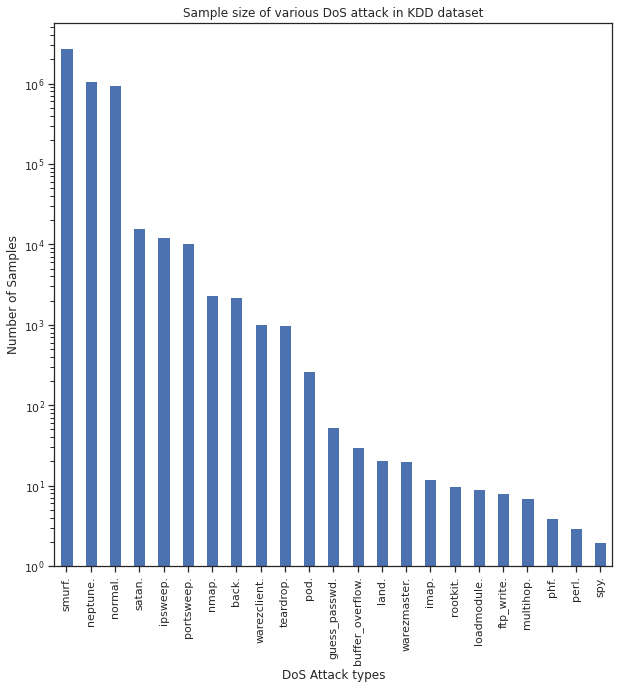
\includegraphics[width=9cm]{KDD_Sample.png}\par
\caption{Plot showing the Number of Samples for Each Attack Type for KDD-CUP-99 dataset.}
\label{samples_kdd}
\end{figure}

In addition, the number of samples for different DoS attack types for NSL-KDD \cite{NSL_kdd} dataset is shown in Figure \ref{samples_nsl}. Here similar to the KDD-CUP-99 dataset the number of samples for each of attack types is not the same and so this dataset like KDD-CUP-99 dataset is unbalanced. 

\begin{figure}[h]
% 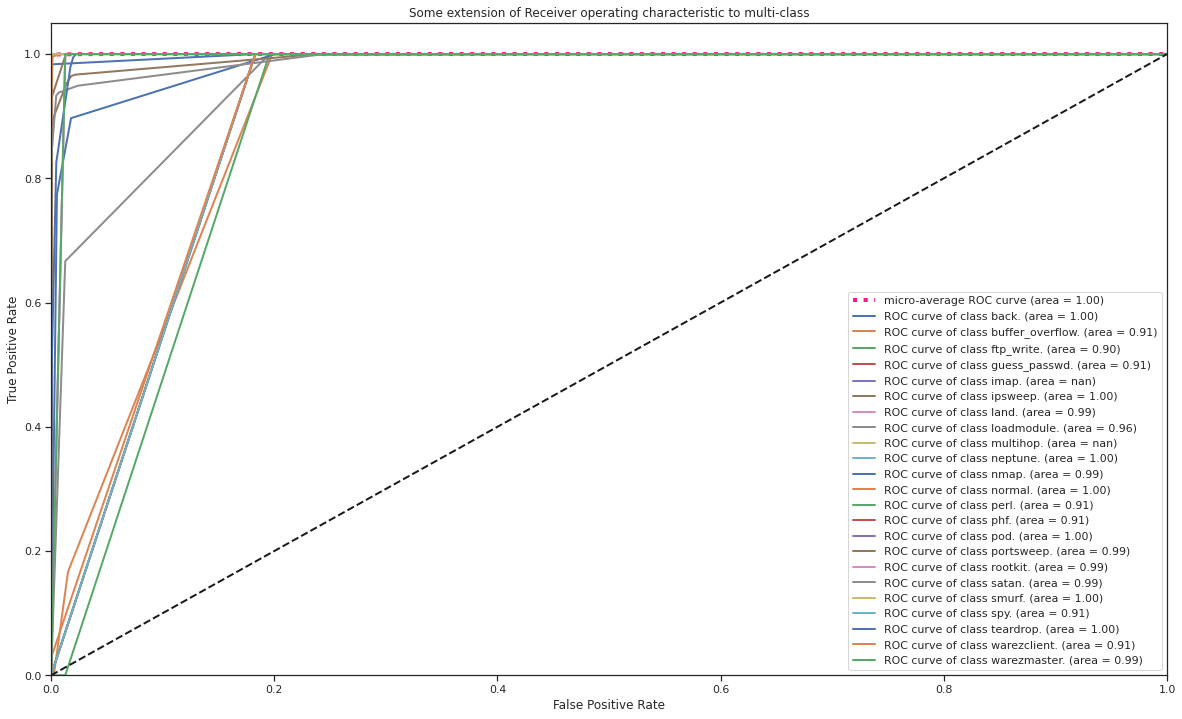
\includegraphics[max size={\textwidth}{\textheight}, angle = 90]{DT_KDD.png}
% \centerline{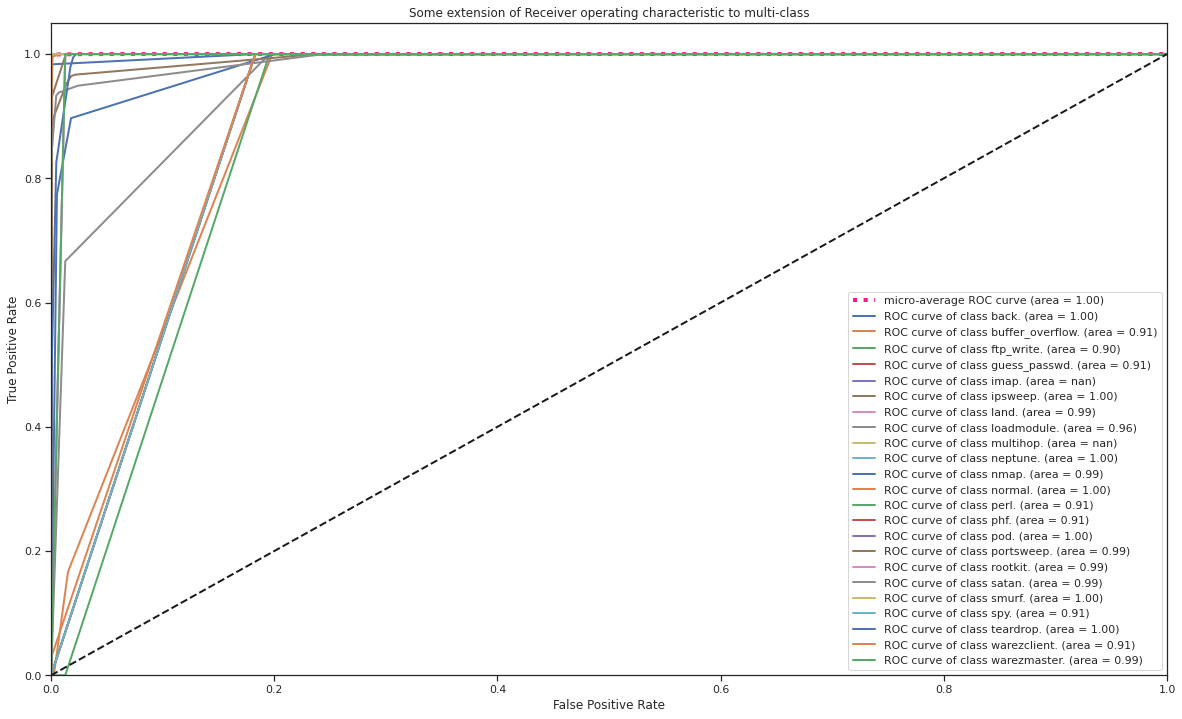
\includegraphics[width=8cm]{DT_KDD.png}}
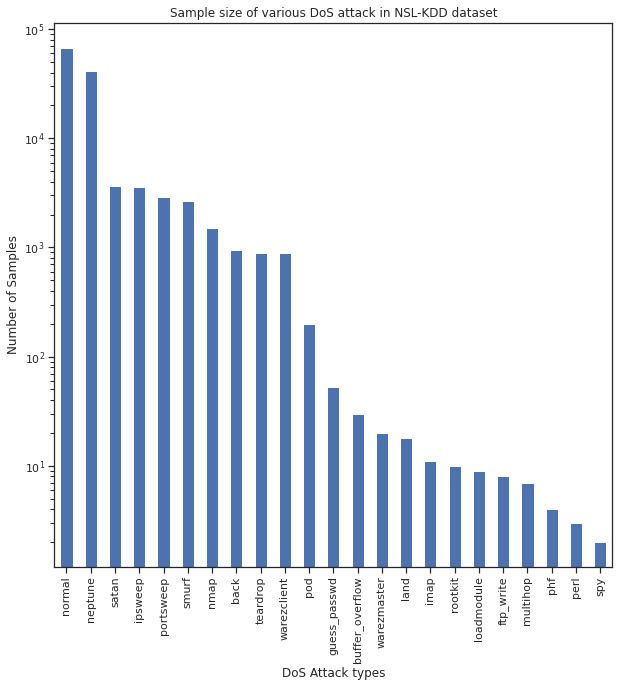
\includegraphics[width=9cm]{NSL_Sample.png}\par
\caption{Plot showing the Number of Samples for Each Attack Type for NSL-KDD dataset.}
\label{samples_nsl}
\end{figure}


\begin{table}[!h]
\centering
\caption{Accuracy Analysis on Models for NSL-KDD dataset}
\label{tab1: Table 3}
\begin{IEEEeqnarraybox}[\IEEEeqnarraystrutmode\IEEEeqnarraystrutsizeadd{2pt}{1pt}]{v/c/v/r/v/c/v}
\IEEEeqnarrayrulerow\\
& \mbox{{\bf Algorithms}} && \mbox{{\bf Accuracy Score}} && \mbox{{\bf Design Parameters}}&\\
\IEEEeqnarraydblrulerow\\
\IEEEeqnarrayseprow[3pt]\\
& \mbox{Random Forest } && \mbox{98.05 \% (Test Set)} && \mbox{$n_{tree} = 1$} &\IEEEeqnarraystrutsize{0pt}{0pt}\\
\IEEEeqnarrayseprow[3pt]\\
\IEEEeqnarrayrulerow\\
\IEEEeqnarrayseprow[3pt]\\
& \mbox{Decision Tree} && \mbox{98.53 \% (Test Set)} && \mbox{$max.\ dept = 15$} &\IEEEeqnarraystrutsize{0pt}{0pt}\\
\IEEEeqnarrayseprow[3pt]\\
\IEEEeqnarrayrulerow\\
\IEEEeqnarrayseprow[3pt]\\
& \mbox{Naive Bayes} && \mbox{61.28 \% (Test Set)} && \mbox{No Parameters} &\IEEEeqnarraystrutsize{0pt}{0pt}\\
\IEEEeqnarrayseprow[3pt]\\
\IEEEeqnarrayrulerow\\
\IEEEeqnarrayseprow[3pt]\\

\IEEEeqnarrayseprow[3pt]\\
& \mbox{MLP} && \mbox{95.83 \% (Test Set)} && \mbox{5 hidden layers
}  &\IEEEeqnarraystrutsize{0pt}{0pt}\\
\IEEEeqnarrayseprow[3pt]\\
\IEEEeqnarrayrulerow\\
\IEEEeqnarrayseprow[3pt]\\


\IEEEeqnarrayseprow[3pt]\\
& \mbox{LSTM} && \mbox{92.32 \% (Test Set)} && \mbox{80x1}  &\IEEEeqnarraystrutsize{0pt}{0pt}\\
\IEEEeqnarrayseprow[3pt]\\
\IEEEeqnarrayrulerow\\
\IEEEeqnarrayseprow[3pt]\\

\IEEEeqnarrayseprow[0.5pt]\\
\IEEEeqnarrayrulerow
\end{IEEEeqnarraybox}
\end{table}





\begin{table}[!h]
\centering
\caption{Accuracy Analysis on Models For KDD-Cup-99 Dataset}
\label{tab1: Table 4}
\begin{IEEEeqnarraybox}[\IEEEeqnarraystrutmode\IEEEeqnarraystrutsizeadd{2pt}{2pt}]{v/c/v/r/v/c/v/}
\IEEEeqnarrayrulerow\\
& \mbox{{\bf Algorithms}} && \mbox{{\bf Accuracy Score}} && \mbox{{\bf Design Parameters}} &\\
\IEEEeqnarraydblrulerow\\
\IEEEeqnarrayseprow[3pt]\\
& \mbox{Random Forest } && \mbox{99.90 \% (Test Set)} && \mbox{$n_{tree} = 5$}  &\IEEEeqnarraystrutsize{0pt}{0pt}\\
\IEEEeqnarrayseprow[3pt]\\
\IEEEeqnarrayrulerow\\
\IEEEeqnarrayseprow[3pt]\\
& \mbox{Decision Tree} && \mbox{99.90 \% (Test Set)} && \mbox{max. Dept = 15} &\IEEEeqnarraystrutsize{0pt}{0pt}\\
\IEEEeqnarrayseprow[3pt]\\
\IEEEeqnarrayrulerow\\
\IEEEeqnarrayseprow[3pt]\\
& \mbox{Naive Bayes} && \mbox{ 92.71 \% (Test Set)} && \mbox{No Parameters}  &\IEEEeqnarraystrutsize{0pt}{0pt}\\
\IEEEeqnarrayseprow[3pt]\\
\IEEEeqnarrayrulerow\\
\IEEEeqnarrayseprow[3pt]\\

\IEEEeqnarrayseprow[3pt]\\
& \mbox{MLP} && \mbox{99.61 \% (Test Set)} && \mbox{5 hidden layers
} &\IEEEeqnarraystrutsize{0pt}{0pt}\\
\IEEEeqnarrayseprow[3pt]\\
\IEEEeqnarrayrulerow\\
\IEEEeqnarrayseprow[3pt]\\


\IEEEeqnarrayseprow[3pt]\\
& \mbox{LSTM} && \mbox{99.32 \% (Test Set)} && \mbox{80x1} &\IEEEeqnarraystrutsize{0pt}{0pt}\\
\IEEEeqnarrayseprow[3pt]\\
\IEEEeqnarrayrulerow\\
\IEEEeqnarrayseprow[3pt]\\

\IEEEeqnarrayseprow[0.5pt]\\
\IEEEeqnarrayrulerow
\end{IEEEeqnarraybox}
\end{table}

\subsection{Naive Bayes}
Naive Bayes \cite{NB} is a supervised Machine Learning algorithm for Binary and multi-class classification that uses Bayes theorem. It is considered a simple or Naive algorithm for information retrieval. Despite its oversimplified assumption, the Naive Bayes algorithm works effectively for many real-world simulations. One of the main advantages of the Naive Bayes algorithm is that training time is quite low for estimating the necessary parameters. As evident from \ref{tab1: Table 1} The training complexity and prediction complexity is lowest among all the other mentioned algorithms in the table. This is the main reason Naive Bayes has been included in this study. The Performance expectation from Naive Bayes is descent and is expected to be lower than that of other algorithms.  

\subsubsection{KDD-CUP-99 Dataset}

The accuracy score for this dataset represents the overall accuracy of all the labels in the test data. The Naive Bayes Classifier accuracy score for this dataset was the lowest among all the three classifiers at 92.71 \%. In addition, there are 6 different class labels for which this classifier's accuracy score is 0\%. Therefore, the Naive Bayes classifier's performance is the lowest among all the mentioned Machine Learning Models.

The results in table \ref{table:05} show the F1-score for all the different types of DoS attacks using the Naive Bayes classifier. It is evident that Naive Bayes \cite{NB} is unable to generalize the different types of attack with a higher F1-score, for example, FtpWrite, Imap, MultiHop, Rootkit and Spy attack types have zero F1-score whereas BufferOverflow, Ipsweep, LoadModule, Nmap, Perl, Portsweep, Satan, WarezClient and Warezmaster have an F1-score below 0.50. There are 7 different attack types for which Naive Bayes gives better F1-score these include Back, Guesspasswd, Neptune, Normal, Pod, Smurf and Teardrop DoS attacks. 


\subsubsection{NSL-KDD Dataset}

The accuracy score is 62.28\% on Test set which quite lower as compared to other Machine Learning algorithms. The performance is lower as compared to KDD-CUP 99 dataset by almost 30\%. This shows that the generalization of Naive Bayes on this dataset is not competitive as compared to other algorithms and gives us a performance that is lowest among all the models on this dataset.    

The F1-score for the NSL-KDD dataset is similar in performance as in KDD-CUP 99 dataset. As shown in table \ref{table:06} there are 6 different DoS attacks for which the F1-score id 0.00 these are FtpWrite, Ipsweep, LoadModule, Perl, Rootkit and Spy which is 5 in the case of KDD-CUP 99 dataset. The attacks that have F1-score less than 0.50 are BufferOverflow, Land, MultiHop, Nmap, Portsweep, Satan, WarezClient and Warezmaster which is similar as in the case above. There are 9 different attack types for which Naive Bayes gives an F1-score greater than 0.50 these include Back, GuessPasswd, Imap, Neptune, Normal, Phf, Pod, Smurf and Teardrop DoS attacks. 

\subsection{Random Forest}

Random Forest \cite{random_forest} is also known by the name of Random Decision Forests which is an Ensemble learning method for Classification and Regression. Random Forest Classifiers often can over-fit the dataset during the training process. It works by splitting each node during the construction of a tree. The best Split can be found by considering the input features or from a random subset of the maximum number of Features. The randomness introduced in the forest gives out decoupled prediction errors. This error is however cancelled out when we take the average of the prediction error. Random Forest Classifier achieves reduced variance with a slight increase in bias as it combines diverse trees. Due to the Variance reduction in Random Forest, the models give out better performance. As from \ref{tab1: Table 1} it is clear that using Random Forest is more Computationally expensive than the other two mentioned algorithms.

\subsubsection{KDD-CUP-99 Dataset}

KDD CUP dataset \cite{KDDcup99} is different from that of the NSL-KDD dataset and in this the major problem that we have encountered is that the dataset doesn't contain enough samples for all the DoS attack types. For example, for rootkit Cyberthreat the dataset contains fewer than 500 samples which are train a Neural Network or a Machine Learning model. The preprocessing of the dataset is the same for the KDD CUP dataset \cite{KDDcup99} as that of the NSL-KDD dataset. The number of features is reduced from 42 to 10 using the Chi2-Squared Test feature selection method. 

In the Random Forest algorithm, the overall validation accuracy on the entire dataset is 99.90 \% when the depth of the tree is 5. Besides, for multiclass classification, the accuracy scores are satisfactory for each of the attack types. However, there are 6 different classes of attacks for which the Random Forest classifier had an accuracy score of 0 \%. One of the main reasons for this is the number of samples available during the testing phase and in each of the cases, the samples were less than 5. Besides, the Prediction Complexity for Random forest is higher than that of both Naive Bayes and Decision Tree Classifiers. 

The F1-score shown in table \ref{table:05} there are 6 different attack types that have an F1-score of 0.00 they are FtpWrite, Imap, LoadModule, Multihop, Rootkit and Spy. However, there is only Land attack type is having an F1-score less than 0.50 which is better than that of the Naive Bayes algorithm. Therefore, in total there are 7 DoS attack types for which Random Forest doesn't have a good F1-score.  

\subsubsection{NSL-KDD Dataset}

The accuracy score for the Random forest algorithm is 98.05\% on the Test set for all the target labels of this dataset when the parameter $n_{tree} = 1$. This accuracy is score is marginally higher than that of the Naive Bayes algorithm. However, this accuracy score is slightly (1.9\%) lower than that of the KDD-CUP-99 dataset.  

The F1-score for this dataset is shown in table \ref{table:06} and the attacks for which the F1-score is zero are FtpWrite, LoadModule, Perl, Rootkit and Spy. In addition similar to the NSL-KDD dataset only Land attack type has an F1-score of less than 0.50. So, there are only 6 different attacks that have a low F1-score which is better than Naive Bayes.

\subsection{Decision Tree}
Decision Trees \cite{CART} are non-parametric supervised learning algorithms that are mainly used for Classification and Regression. It predicts the targets by learning decision rules inferred from the input features without using any parameters. Decision trees require little data preparation however it can create overly complex trees which in some cases leads to overfitting and then the generalization of the dataset decreases. As from \ref{tab1: Table 1} the prediction complexity is similar to that of Naive Bayes algorithm \cite{NB} however its Training Complexity is higher than Naive Bayes.   

\subsubsection{KDD-CUP-99 Dataset}

In the Case of Decision Tree Classifier, the accuracy score for the validation test is 99.90 \% which is identical to that of the Random Forest Classifier. However, in this case, also there were 6 different classes for which the Classifier didn't give any accuracy score. One key point to note is that the Prediction Complexity of Decision Tree is less than that of Random forest Classifier by a factor of $n_{trees}$ which makes Decision Tree Classifier efficient than Random Forest Classifier.  

The F1-score for KDD-CUP-99 Dataset using the Decision Tree algorithm is shown in table \ref{table:05}. The attack types FtpWrite, Imap, LoadModule, MultiHop, Perl, Phf, Spy and warezmaster all have an F1-score of 0.00. In addition, only the Land attack type has an F1-score of less than 0.50 rest all other attacks have an F1-score of more than 0.50 and this number for this dataset using the Decision Tree algorithm is 15 which is lower than Random Forest for the same dataset.

\subsubsection{NSL-KDD Dataset}

The Accuracy Score for NSL-KDD dataset \cite{KDDcup99} for Decision Tree is 98.53\% which is highest among all the models presented in Table \ref{tab1: Table 3}. The Decision tree's performance is dependent on the dept of the Tree and for this dataset to achieve the best performance for all the attack types the maximum depth of the tree is kept to be 15 which is shown in Table \ref{tab1: Table 3}. The maximum depth of the tree does not affect the computational complexity of the algorithm which is an advantage over other algorithms.   

F1-Score Analysis: 
The F1-score for this dataset is shown in table \ref{table:06}. It is evident that there are 4 different attack types for which F1-score is 0.00, they are FtpWrite, Perl, Rootkit and Spy. This number is the lowest among all the mentioned Machine Learning Algorithms. In addition, the attacks Land and LoadModule have an F1-score of less than 0.50. which is similar in performance to that of the Random Forest algorithm. So, the Decision Tree has only 6 different attack types for which the F1-score is below 0.50 rest all have a score above 0.50 which 17 in this case.  

\subsection{MultiLayer Perceptron}
Multilayer Perceptron \cite{MLP} (MLP) is a supervised learning algorithm that uses Backpropagation learning method \cite{MLP} by learning a function $ f(\cdot): R^{f} \rightarrow R^{o}$ by training procedure on the dataset. Here $f$ is the number of input features and $o$ is the number of class labels. It has the ability to learn non-linear functions in real-time (on-line learning) which increases the application area for MLP. However, it needs proper optimization algorithms due to its concave loss function along with tuning for hyperparameters such as layers, hidden neurons and number of iterations for training. It has the capability for Multi-class classification by using the Softmax activation function on its output layer. 

\subsubsection{KDD-CUP-99 Dataset}

There are only two Deep Neural Network (DNN) models chosen for this problem as there other seems to be more Computationally expensive. In the first case, an MLP with 3 hidden layers (100*50*25) was chosen for the Multiclass Classification problem. This model gave an accuracy score of 99.61 \% for the overall dataset. However, there were 11 different Classes for which the model was not able to predict sufficient accuracy score. The main problem is again the low number of samples in the dataset for each of these classes.\par

The F1 score for various types of DoS attack is given in Table \ref{table:05} for MLP classifier. For some of the DoS attack types, the F1 score is very low which means poor precision and recall for that particular class. For MLP classifier, Neptune, Pod, Smurf and WarezClient have the highest F1 score while BufferOverflow, FtpWrite, GuessPasswd are among the ones who have an F1 score of zero. The F1 score for various DoS attack types tends to be either near 1 or zero with the only exception of Portsweep.   

\subsubsection{NSL-KDD Dataset}

The MLP used for NSL-KDD Dataset has 3 hidden layers (100*50*25) with softmax as activation function at the output layer. The classifier gave an overall accuracy of 96 \%.  Though the overall accuracy is satisfactory, the classifier was unable to correctly classify 8 types of DoS attacks out of 23 types. Since the NSL-KDD Dataset has less number of samples compared to KDD-CUP-99 Dataset, the performance of MLP classifier on NSL-KDD Dataset is poor compared to KDD-CUP-99 Dataset.

The F1 score using an MLP classifier for various types of DoS attacks has been shown in Table \ref{table:06}. The F1 for some of the DoS attacks is above 80 \% which includes Back, GuessPasswd, Ipsweep, Neptune, Pod, Satan, Smurf, Teardrop, WarezClient and Warezmaster. But the classifier was unable to correctly identify some of DoS attacks which resulted in a lower F1 score for BufferOverflow, FtpWrite, Imap, Land, LandModule, Multihop etc.

\subsection{Long Short Term Memory}
Long Short Term Memory (LSTM) \cite{lstm} is based on Recurrent Neural Network (RNN) architecture that is majorly used in Deep learning with feedback connections which is different from that of Feedforward Neural Networks. LSTM works well for classification, processing and making predictions on time-series datasets. It was mainly developed to overcome the Vanishing and Exploding gradient problem encounter in RNN architecture. The design of the LSTM network used in this scenario for both the dataset has 80 LSTM units and 1 dense layer with 23 units in it for classifying the different DoS attack types. 


\subsubsection{KDD-CUP-99 Dataset}

LSTM has a high accuracy score of 99.32\% on Test set for the targets which contain all the different attack labels. This score is slightly lower than MLP but better than Naive Bayes which has the lowest accuracy score of 92.71\% among all the algorithms.

The F1-score for this dataset using LSTM is shown in table \ref{table:05}. The attack types which have an F1-score of 0.00 are BufferOverflow, FtpWrite, Imap, Land, LoadModule, MultiHop, Nmap, Perl, Phf, Rootkit and Spy which higher than MLP. In addition, the attacks which have an F1-score less than 0.50 are GuessPasswd, Portsweep and WarezClient. Apart from these attacks, all the other attacks have an F1-score greater than 0.50. Besides, only a few of the attack types such as Neptune, Satan and Smurf have a perfect F1-score of 1.00 given out by the model.  

\subsubsection{NSL-KDD Dataset}

The Accuracy Score of NSL-KDD for LSTM is 92.32\% which shown in table \ref{tab1: Table 3}. This score is lower than that of the KDD-CUP-99 dataset by 7\% for the same number of LSTM units. The LSTM classifier has 80 hidden units with a dense layer having 500 neurons. The Dropout layer has also been added which allows the neuron to work independently instead of being dependent on a small number of neurons.

The F1 score using an LSTM classifier for various types of DoS attacks has been shown in Table \ref{table:06}. Some of the attack types have 0 F1 scores which are FtpWrite, Land, LandModule, MultiHop, Perl, Phf and Spy. This result is similar to KDD-CUP-99 Dataset with LSTM classifier with some improvement for some attack types in terms of F1 score. For the LSTM classifier, Back, GuessPasswd, Imap, Ipsweep, Neptune, Pod attack types have the highest accuracy score.


\begin{table*}
\caption{Accuracy Score for Different Algorithm on KDD-CUP-99 Dataset}
\label{table:05}
\begin{tabularx}{\textwidth}{@{}l*{22}{C}c@{}}
\toprule
\bf CyberAttacks  & \bf Naive Bayes (F1 Score)  & \bf Random Forest (F1 Score) & \bf Decision Tree (F1 Score) & \bf MLP (F1 Score) & \bf LSTM (F1 Score) \\ 
\midrule
Back            & 0.99      & 1.00          & 1.00    & 0.93       & 0.90 \\
BufferOverflow  & 0.01      & 0.67          & 0.67    & 0.00       & 0.00 \\ 
FtpWrite        & 0.00      & 0.00          & 0.00    & 0.00       & 0.00 \\
GuessPasswd     & 0.86      & 0.95          & 1.00    & 0.00       & 0.20 \\ 
Imap            & 0.00      & 0.00          & 0.00    & 0.00       & 0.00 \\ 
Ipsweep         & 0.02      & 0.97          & 0.96    & 0.89       & 0.88 \\ 
Land            & 0.01      & 0.33          & 0.33    & 0.00       & 0.00 \\ 
LoadModule      & 0.07      & 0.00          & 0.00    & 0.00       & 0.00 \\ 
MultiHop        & 0.00      & 0.00          & 0.00    & 0.00       & 0.00 \\ 
Neptune         & 0.98      & 1.00          & 1.00    & 1.00       & 1.00 \\ 
Nmap            & 0.02      & 0.50          & 0.87    & 0.00       & 0.00 \\ 
Normal          & 0.81      & 1.00          & 1.00    & 0.99       & 0.99 \\ 
Perl            & 0.13      & 1.00          & 0.00    & 0.00       & 0.00 \\ 
Phf             & 1.00      & 1.00          & 0.00    & 0.00       & 0.00 \\ 
Pod             & 0.76      & 0.99          & 0.98    & 1.00       & 0.96 \\ 
Portsweep       & 0.08      & 0.88          & 0.85    & 0.56       & 0.42 \\ 
Rootkit         & 0.00      & 0.00          & 1.00    & 0.00       & 0.00 \\ 
Satan           & 0.01      & 0.96          & 0.99    & 0.90       & 1.00 \\ 
Smurf           & 1.00      & 1.00          & 1.00    & 1.00       & 1.00 \\ 
Spy             & 0.00      & 0.00          & 0.00    & 0.00       & 0.00 \\ 
Teardrop        & 1.00      & 1.00          & 1.00    & 0.94       & 0.99 \\ 
WarezClient     & 0.08      & 0.98          & 0.99    & 1.00       & 0.49 \\ 
Warezmaster     & 0.02      & 0.00          & 0.00    & 0.00       & 0.50 \\ 


\bottomrule
\end{tabularx}
\end{table*}




\begin{table*}
\caption{Accuracy Score for Different Algorithm on NSL-KDD Dataset}
\label{table:06}
\begin{tabularx}{\textwidth}{@{}l*{22}{C}c@{}}
\toprule
\bf CyberAttack Types & \bf Naive Bayes (F1 Score)  & \bf Random Forest (F1 Score) & \bf Decision Tree (F1 Score) & \bf MLP (F1 Score) & \bf LSTM (F1 Score) \\ 
\midrule
Back            & 0.98      & 1.00   & 0.99         & 0.95    & 0.95  \\ 
BufferOverflow  & 0.25      & 0.77   & 0.67         & 0.00    & 0.57   \\ 
FtpWrite        & 0.00      & 0.00   & 0.00         & 0.00    & 0.00   \\ 
GuessPasswd     & 0.77      & 0.92   & 0.86         & 0.81    & 0.93  \\ 
Imap            & 1.00      & 1.00   & 1.00         & 0.00    & 1.00 \\ 
Ipsweep         & 0.00      & 0.91   & 0.92         & 0.85    & 0.81  \\ 
Land            & 0.01      & 0.40   & 0.40         & 0.00    & 0.00 \\ 
LoadModule      & 0.00      & 0.00   & 0.40         & 0.00    & 0.00  \\ 
MultiHop        & 0.08      & 1.00   & 0.67         & 0.00    & 0.00  \\ 
Neptune         & 0.91      & 0.99   & 0.99         & 0.98    & 0.97   \\ 
Nmap            & 0.09      & 0.62   & 0.66         & 0.17    & 0.17  \\ 
Normal          & 0.60      & 1.00   & 1.00         & 0.98    & 0.97  \\ 
Perl            & 0.00      & 0.00   & 0.00         & 0.00    & 0.00   \\ 
Phf             & 1.00      & 1.00   & 1.00         & 0.00    & 0.00  \\ 
Pod             & 0.95      & 0.99   & 0.99         & 0.99    & 0.99 \\ 
Portsweep       & 0.39      & 0.87   & 0.89         & 0.73    & 0.70  \\ 
Rootkit         & 0.00      & 0.00   & 0.00         & 0.00    & 0.00 \\ 
Satan           & 0.09      & 0.92   & 0.93         & 0.81    & 0.74  \\ 
Smurf           & 0.99      & 1.00   & 1.00         & 1.00    & 0.99  \\ 
Spy             & 0.00      & 0.00   & 0.00         & 0.00    & 0.00   \\ 
Teardrop        & 0.99      & 1.00   & 1.00         & 1.00    & 1.00  \\ 
WarezClient     & 0.29      & 0.99   & 0.97         & 0.81    & 0.73   \\ 
Warezmaster     & 0.44      & 0.86   & 0.86         & 0.86    & 0.86  \\ 


\bottomrule
\end{tabularx}
\end{table*}


\section{Discussion}
In this section we discuss the results obtained on the two different datasets \cite{KDDcup99} mentioned in the previous section. The Naive Bayes Classifier \cite{NB} has an accuracy score of 61.28\% on the Test set for the NSL-KDD dataset \cite{KDDcup99} which is the lowest score among all the model mentioned in table \ref{tab1: Table 3}. In addition, the accuracy score on the KDD-CUP-99 dataset is improved by 30\% to 92.71\% on the test set. However, this score is the lowest accuracy score among all the models for the KDD-CUP-99 dataset. One major reason for the improvement in the performance of the algorithm is mainly due to the increase in the number of samples in the KDD-CUP-99 dataset which is far greater than the NSL-KDD dataset. The F1-score for Naive Bayes on the two datasets is similar and in both the datasets there are attacks for which the F1-score is 0.00 these are those attacks for which the number of samples in the dataset is very low. In some cases, there were no samples of the attack types in the test set while testing the Classifier on the dataset. However, the generalization of this classifier was less compared to other models in both the datasets. The RoC curve for the Naive Bayes algorithm on KDD-CUP-99 and NSL-KDD dataset is shown in figure \ref{NB_KDD} and \ref{NB_NSL} respectively. In figure \ref{NB_KDD} there are some attack types for which the area under the curve is below the imaginary line which shows that the classifier doesn't perform well for those attack types. Besides, most of the attack types reside on the upper left corner of the graph which tells us that on this dataset the performance is acceptable. In contrast, Figure \ref{NB_NSL} performance is lower as the area under curve decrease and in this case, the algorithm behaves far from ideal. However, One advantage of the Naive Bayes algorithm is its low training and prediction Complexity that makes it an efficient algorithm but the generalization, in this case, is poor. Therefore, the Naive Bayes algorithm is not an ideal model for the multiclass classification of KDD-CUP-99 and NSL-KDD datasets \cite{KDDcup99}.

The second model is the Random Forest algorithm \cite{random_forest} and the accuracy score for the KDD-CUP-99 and NSL-KDD dataset is 99.90\% and 98.05\% respectively when the design parameter of $n_{trees} = 5$ is chosen. When the design parameter is altered the accuracy score of the multiclass classification for the algorithm decreases which in turn affects the detection of different attack types using this algorithm. In addition, the F1-score for the datasets shows us that for each of the attack types the algorithm performs better than Naive Bayes \cite{NB} algorithm. The F1-score from the KDD-CUP-99 dataset it is clear that the overall performance in predicting the attack types has improved significantly when compared to the Naive Bayes algorithm. For example, the F1-score in detecting the BufferOverflow has improved from 0.01 by Naive Bayes to 0.67 in Random Forest which effectively tells us that the attack is BufferOverflow attack and this can be said with more precision in the case of Random Forest algorithm. The RoC curve obtained in figure \ref{RF_KDD} has a better area under the curve than that of Naive Bayes however for some classes the area under the curve is lower. In comparison, Figure \ref{Rf_NSL} obtained on the NSL-KDD dataset has more number of classes for which the area under the curve is lower which shows that the performance of Random Forest decreases in the case of NSL-KDD dataset which is still better than that of Naive Bayes algorithm. Besides, the Training complexity of the Random Forest algorithm as mentioned in Table \ref{tab1: Table 1} is highest among all the mentioned Machine Learning models. 

Decision Tree \cite{CART} has an identical accuracy score to that of Random Forest \cite{random_forest} in the case of the KDD-CUP-99 dataset which is highest among all the algorithm. The performance in the case of NSL-KDD is slightly better which makes it the ideal algorithm for multi-class classification for the NSL-KDD dataset. One important point to consider is that the maximum depth of the tree is 15 which is an important parameter in order to achieve maximum performance from this algorithm for this particular dataset. Decision Tree has the best F1-scores for the different attack types among the algorithms in the NSL-KDD dataset. As shown in Table \ref{table:06} It has only 4 different attack types for which the F1-score is 0.00 and in two of the cases there were no test samples in the test set which is the lowest among all the presented algorithms. For the KDD-CUP dataset, the performance of the Decision Tree is almost identical to the Random forest and in some cases, it is better. For example, in Nmap the F1-score increases from 0.50 in Random forest to 0.87 in Decision Trees. One of the main reasons for low F1-score in some cases is because both the dataset is unbalanced and in some cases, lack of adequate samples makes it difficult for the classifier to classify the different attack types. The RoC curve for Decision Tree is shown in figure \ref{DT_KDD} and \ref{DT_NSL} for KDD-CUP-99 and NSL-KDD dataset respectively. The area under the curve for the KDD-CUP-99 dataset is much higher than any of the other classifiers mentioned. In comparison, the area under the curve for the NSL-KDD dataset is lower and the generalization is better than the Random Forest algorithm. Besides, one major advantage of the Decision Tree algorithm is that the prediction Complexity is the same as that of the Naive Bayes algorithm which makes it an efficient high-performance algorithm for multiclass classification for DoS attacks type detection in Sensor Networks. 

In the first of Artificial Intelligence (AI) Models, MLP is used and the accuracy score for it on the KDD-CUP-99 dataset is 99.61\% on the test set. Besides, the accuracy score on the NSL-KDD dataset is 95.83\% which is lower than that of the KDD-CUP-99 dataset. MLP has the highest accuracy score between the two AI models and its performance is similar to the Machine Learning algorithms. In addition, the F1-score obtained for different DoS attacks KDD-CUP-99 dataset is poor. It has an F1-score of 0.00 for 13 different attack types which the worst performance amongst all the models presented. However, the performance on NSL-KDD is better and has a lower number of attack types which has an F1-score of 0.00. The RoC curve is shown in Figure \ref{MLP_KDD} and \ref{MLP_NSL} for KDD-CUP-99 dataset and NSL-KDD dataset. The area under the curve in Figure \ref{MLP_KDD} is lower for some class labels for eg. WarezMaster attack the area is only 0.78. However, in comparison, this performance gets better on the NSL-KDD dataset in which is clear that the area under the curve is higher than that from Figure \ref{MLP_KDD} which aligns with the F1-score performance and Accuracy score for each of the dataset. Besides, MLP has a large Memory requirement for storing trained parameters to do an effective prediction. The prediction complexity of MLP is higher than that of Machine Learning models which is a drawback in the case where efficiency is of paramount importance.

The second AI model used for Multi-class classification is LSTM and the accuracy score on the KDD-CUP-99 dataset is 99.32\% which is slightly lower than MLP for the same case. The score decreases by almost 7\% for the NSL-KDD datasets. The F1-score presented in table \ref{table:05} is for the KDD-CUP-99 dataset and this score is similar to MLP with a low number of attack types which has an F1-score of 0.00. The F1-score for NSL-KDD is shown in table \ref{table:06} and the score is better than that in table \ref{table:05}. For eg. the attack type Warezmaster has an F1-score of 0.50 in the KDD-CUP-99 dataset and an F1-score of 0.86 in the case of the NSL-KDD dataset which is far better. In comparison to MLP, the score is similar in some cases whereas lower in some cases. The RoC curve for LSTM is shown in Figure \ref{LSTM_KDD} and \ref{LSTM_NSL} for KDD-CUP-99 and NSL-KDD dataset. The Performance-based on RoC curve for KDD-CUP-99 shows that LSTM performs better than MLP when compared to all the classes as the area under the curve is higher for LSTM than that in Figure \ref{MLP_KDD} which shows RoC curve for MLP on KDD-CUP-99 dataset. However, the case is not similar for the NSL-KDD dataset when the RoC curve is compared between LSTM and MLP. The area under the curve if lower for the majority of the attack types in Figure \ref{LSTM_NSL} than that of Figure \ref{MLP_NSL}. In addition, the generalization for the two datasets using LSTM is not as expected given the Computation complexity for the algorithm. Besides, this performance of LSTM is lower for Multiclass classification when compared to more efficient Machine Learning models presented in Table \ref{tab1: Table 1}. 

\section{Conclusion}
A study of 5 different models was presented based on the Training and Prediction complexity of the algorithms and the analysis on each one for the KDD-CUP-99 and NSL-KDD dataset was performed in the discussion section. The Multi-class classification for each of the models was performed and the F1-score for detecting each of the attack types for the two datasets was presented in table \ref{table:05} and \ref{table:06}. The accuracy score presented in table \ref{tab1: Table 3} and \ref{tab1: Table 4} for NSL-KDD and KDD-CUP-99 dataset is the overall accuracy score for the complete target set which consists of all the attack types. This detailed analysis of multi-class classification was lacking in all the papers that we reviewed for DoS Intrusion detection in Wireless Sensor Networks in section II.

For efficient model selection, 5 different AI and ML models were presented. Among the AI and ML models, it is evident that the ML Models outperform the AI models in terms of Accuracy score, F1-score and RoC curve analysis for Multiclass classification for both the datasets. The results discussed in the above section show that among the 3 presented Machine Learning Models Naive Bayes and Decision Tree has the lowest Prediction Complexity and then we have Random Forest which has higher Prediction Complexity than the two algorithms. The metrics for Naive Bayes on the two different dataset \cite{KDDcup99} shows that it is not an ideal algorithm for Multiclass classification for a different kind of DoS Intrusion detection. The performance between Random Forest \cite{random_forest} and Decision Tree \cite{CART} is similar when compared with the three metrics given above and in some cases of attack types, Decision Tree tends to outperform Random Forest by some good margin.  In addition, Decision Tree has lower Prediction Complexity when compared with that of the Random Forest algorithm which makes it an ideal and efficient classifier as lower complexity means low power and memory requirement from Wireless Sensor Network for performing Multi-class classification and detecting all different kinds of DoS intrusion detection.

% \begin{figure}[htbp]
% % 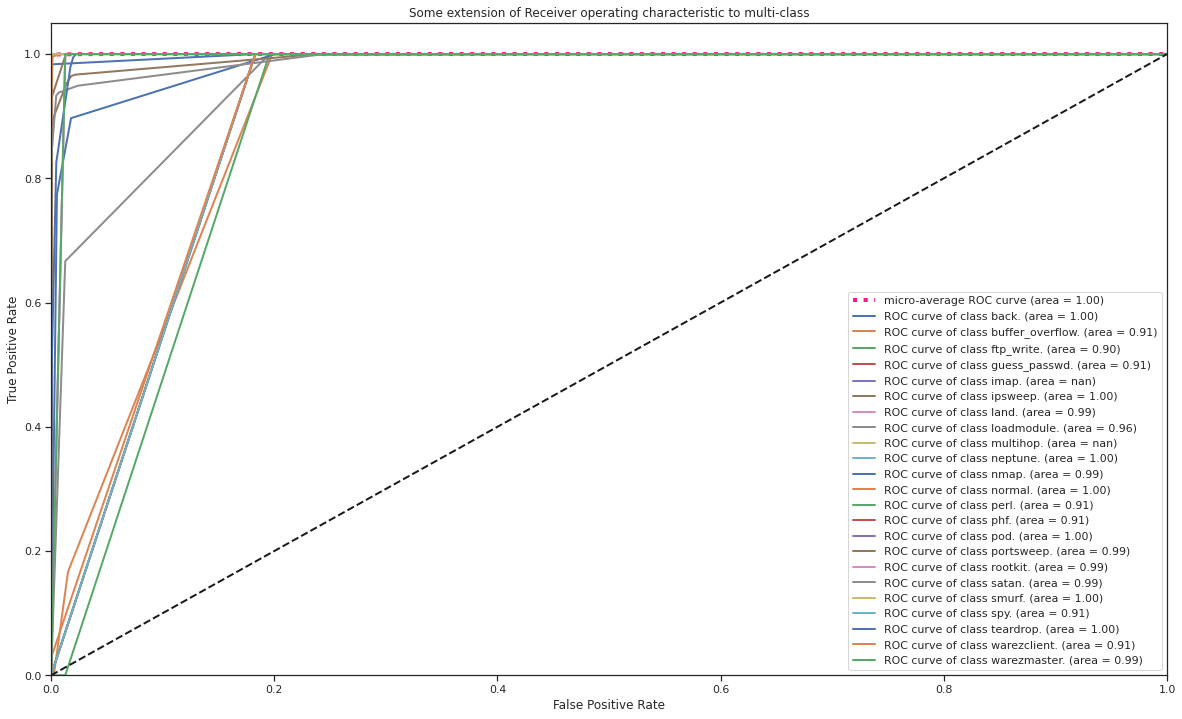
\includegraphics[max size={\textwidth}{\textheight}, angle = 90]{DT_KDD.png}
% \centerline{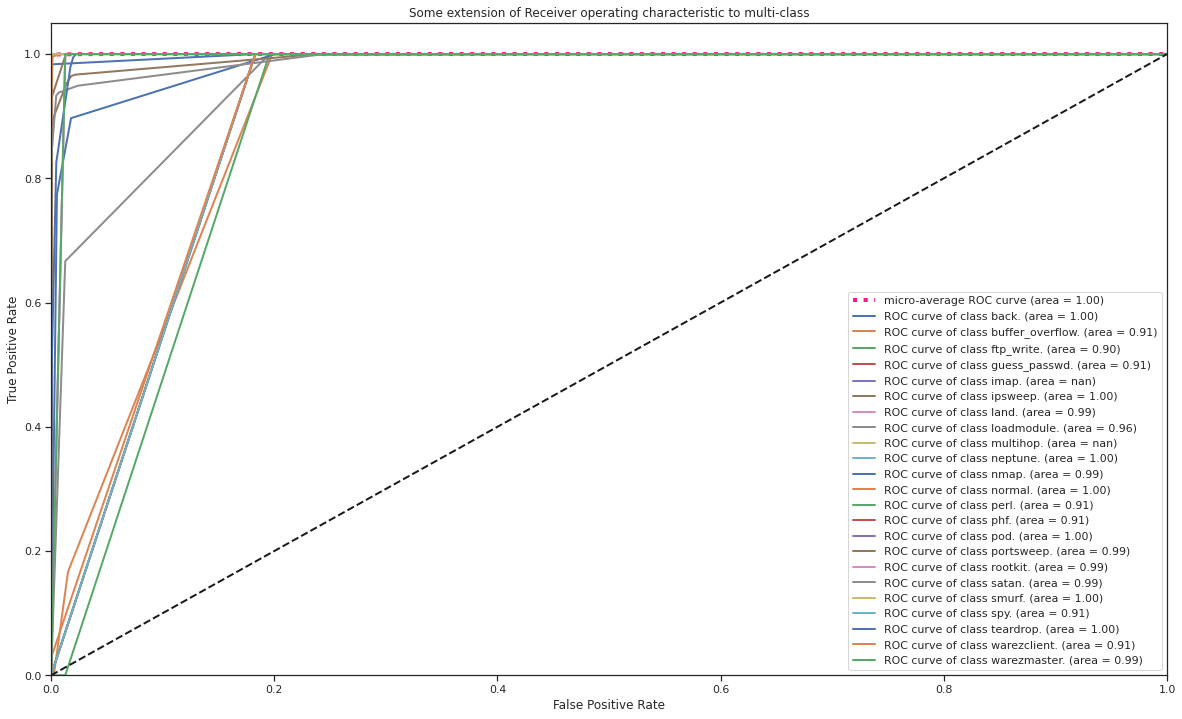
\includegraphics[width=8cm]{DT_KDD.png}}
% \caption{RoC curve for Decision Tree for KDD-CUP-99 Dataset.}
% \label{DT_KDD}
% \end{figure}


\clearpage
\begin{figure}[ht!]
  \centering
  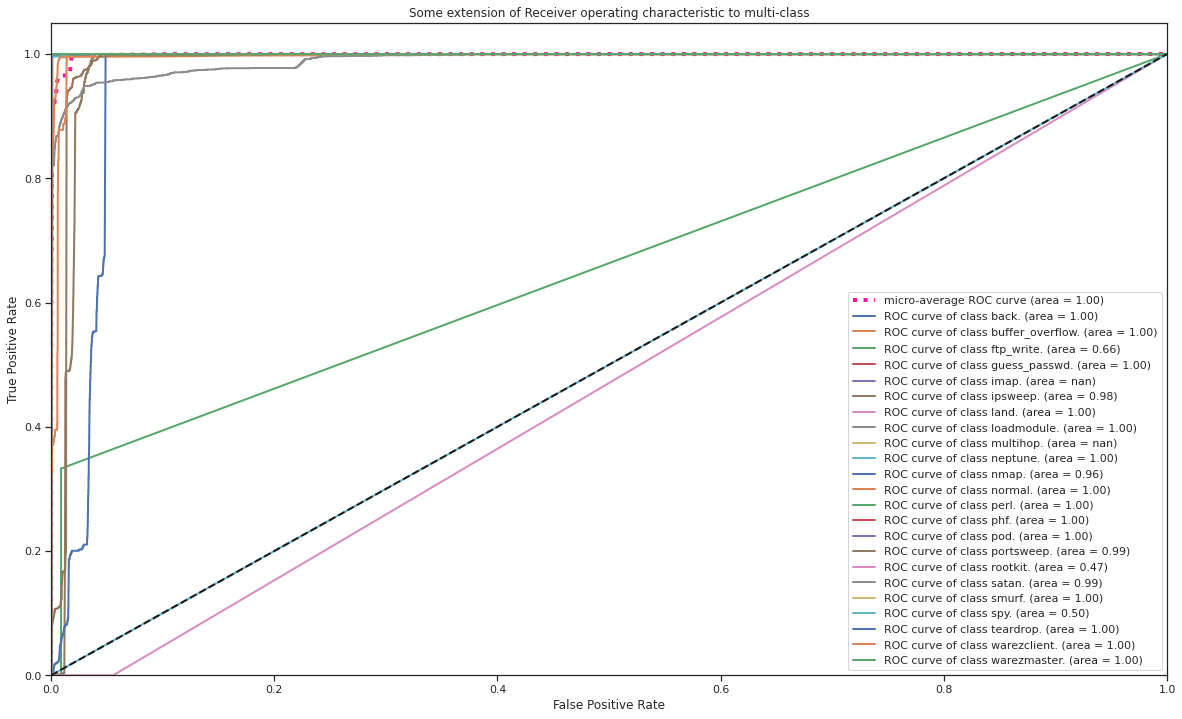
\includegraphics[width=18cm]{GNB_KDD.png}
  \caption{RoC curve of Naive Bayes on KDD-CUP-99 Dataset}
  \label{NB_KDD}

  \vspace*{\floatsep}% https://tex.stackexchange.com/q/26521/5764

  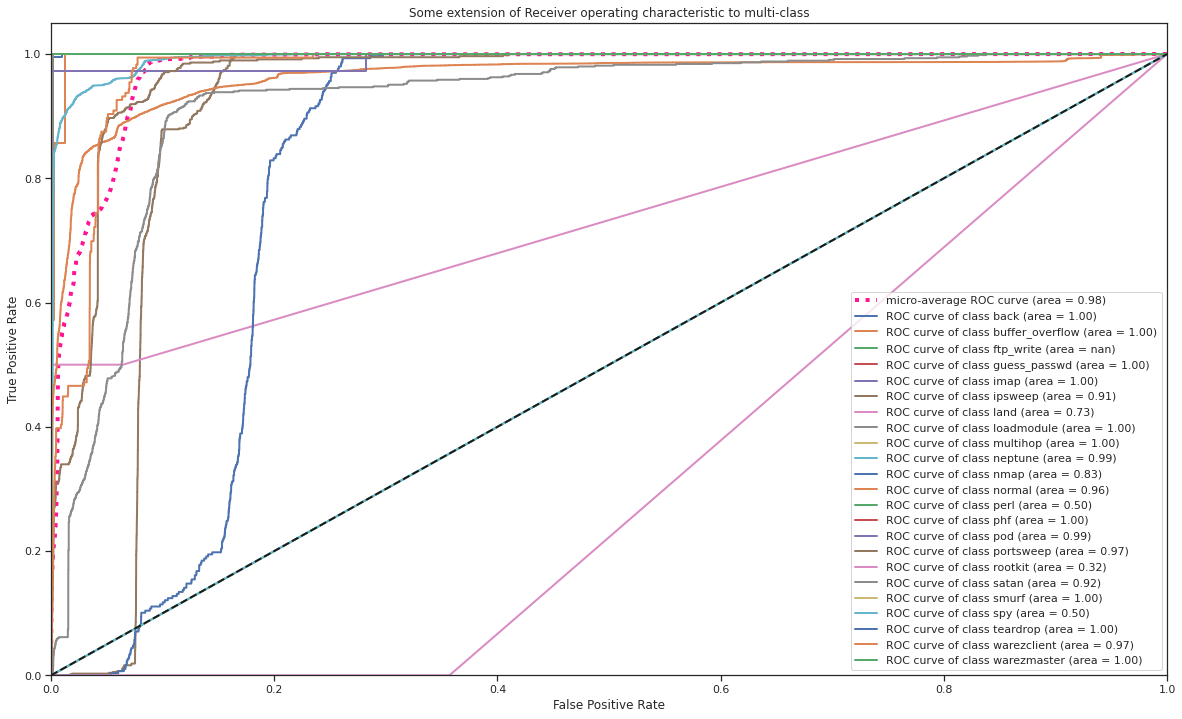
\includegraphics[width=18cm]{GNB_NSL.png}
  \caption{RoC curve of Naive Bayes on NSL-KDD Dataset}
  \label{NB_NSL}
  
\end{figure}

\clearpage
\begin{figure}[h]
  \centering
  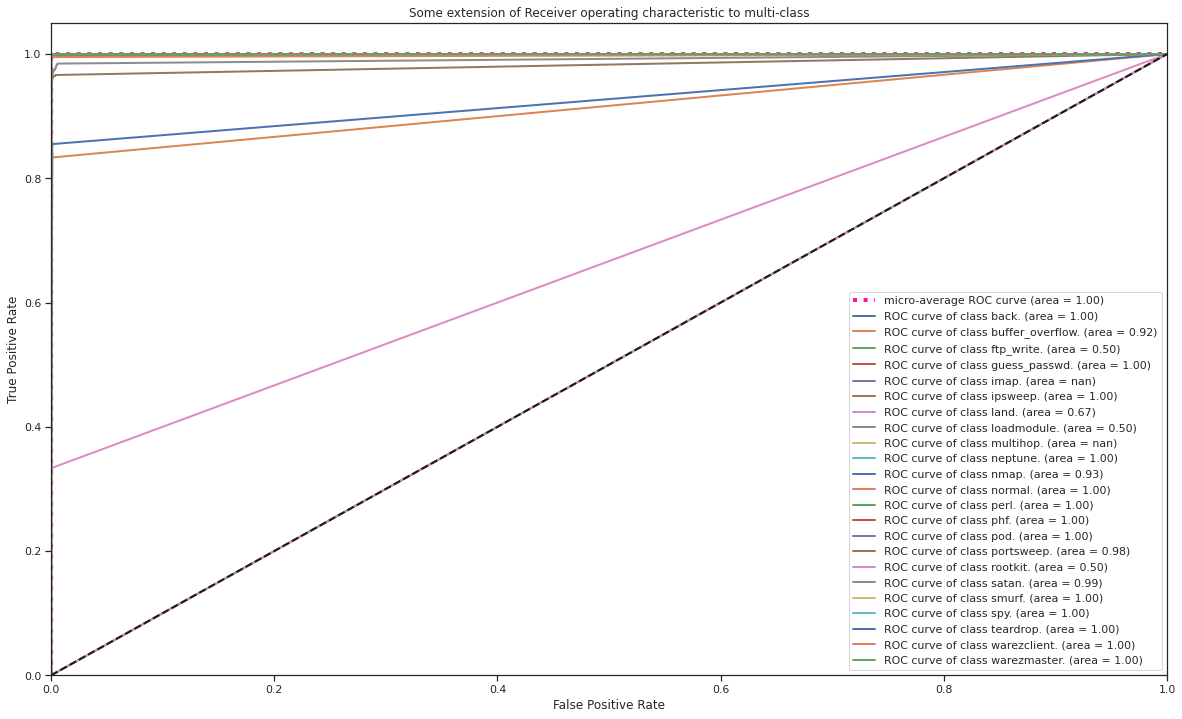
\includegraphics[width=18cm]{RF_KDD.png}
  \caption{RoC curve of RF on KDD-CUP-99 Dataset}
  \label{RF_KDD}

  \vspace*{\floatsep}% https://tex.stackexchange.com/q/26521/5764

  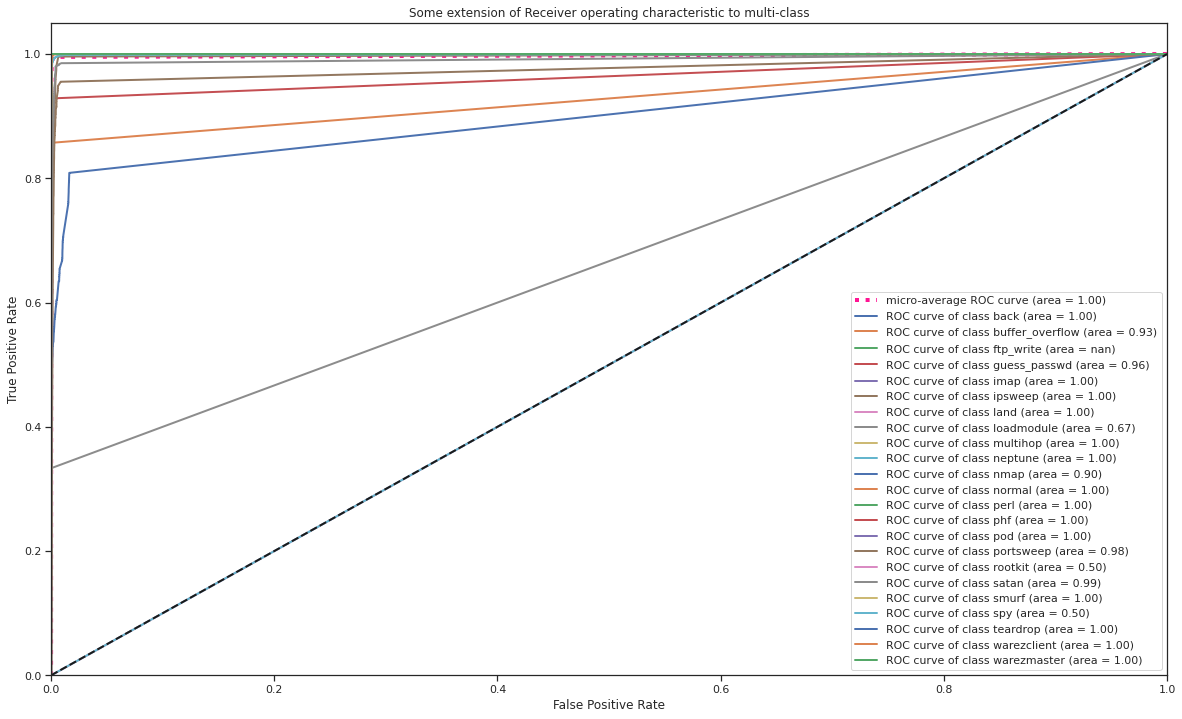
\includegraphics[width=18cm]{RF_NSL.png}
  \caption{RoC curve of RF on for NSL-KDD Dataset}
  \label{Rf_NSL}
  
\end{figure}

\clearpage
\begin{figure}[h]
  \centering
  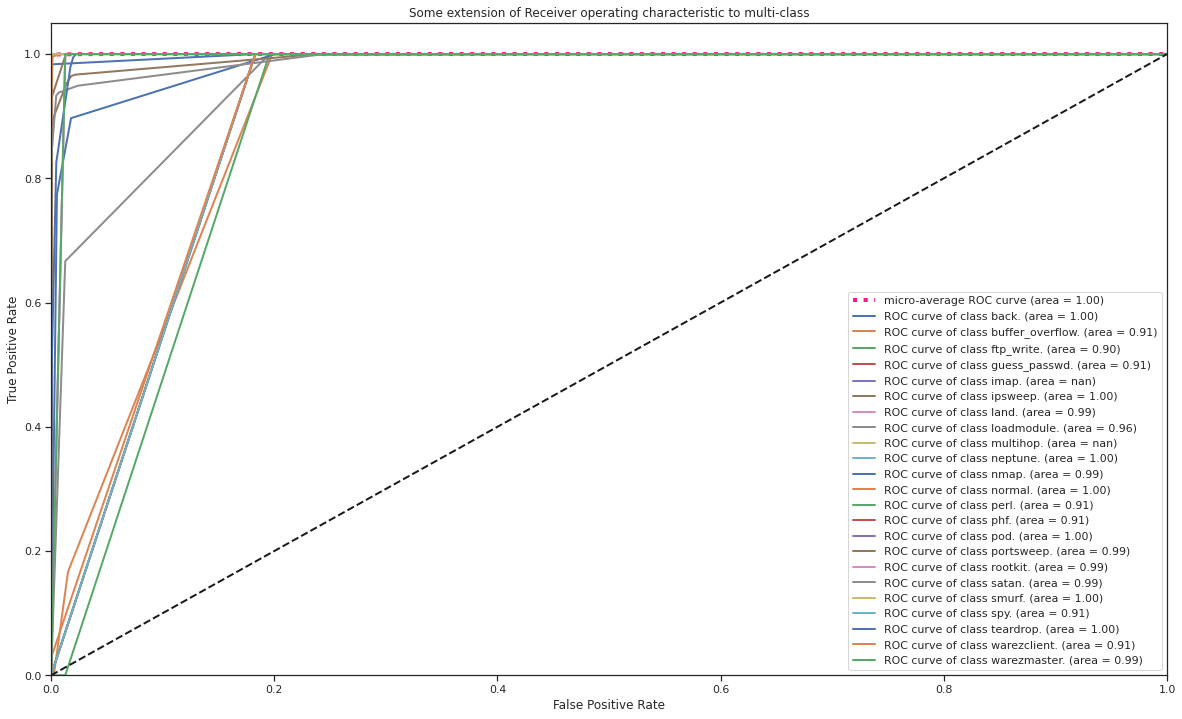
\includegraphics[width=18cm]{DT_KDD.png}
  \caption{RoC curve of Decision Tree on KDD-CUP-99 Dataset}
  \label{DT_KDD}
  \vspace*{\floatsep}% https://tex.stackexchange.com/q/26521/5764

  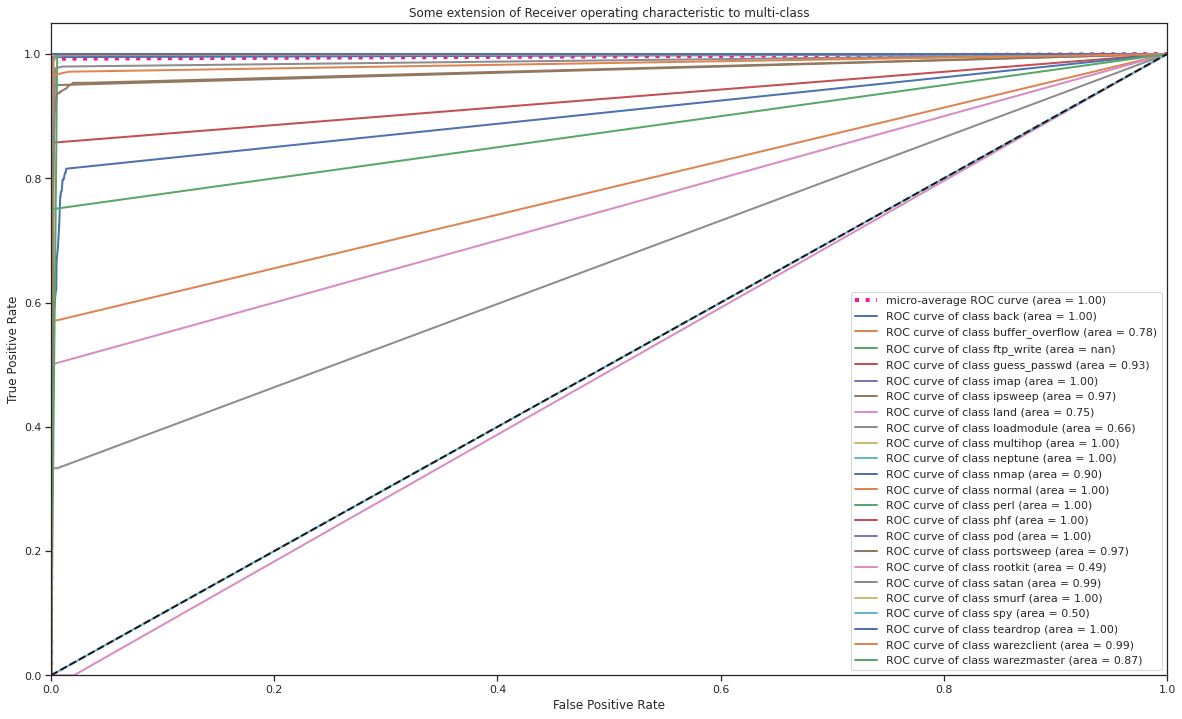
\includegraphics[width=18cm]{DT_NSL.png}
  \caption{RoC curve of Decision Tree on NSL-KDD Dataset}
  \label{DT_NSL}
\end{figure}

\clearpage
\begin{figure}[h]
  \centering
  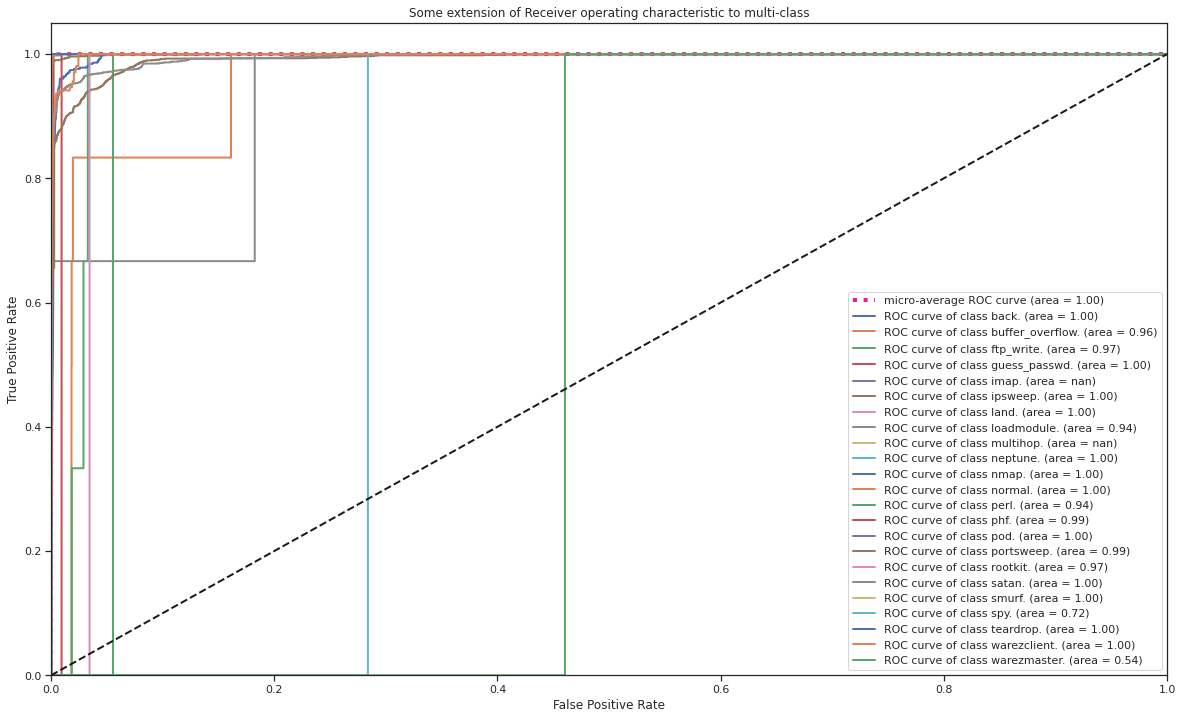
\includegraphics[width=18cm]{MLP_KDD.png}
  \caption{RoC curve of MLP on KDD-CUP-99 Dataset}
  \label{MLP_KDD}
  \vspace*{\floatsep}% https://tex.stackexchange.com/q/26521/5764

  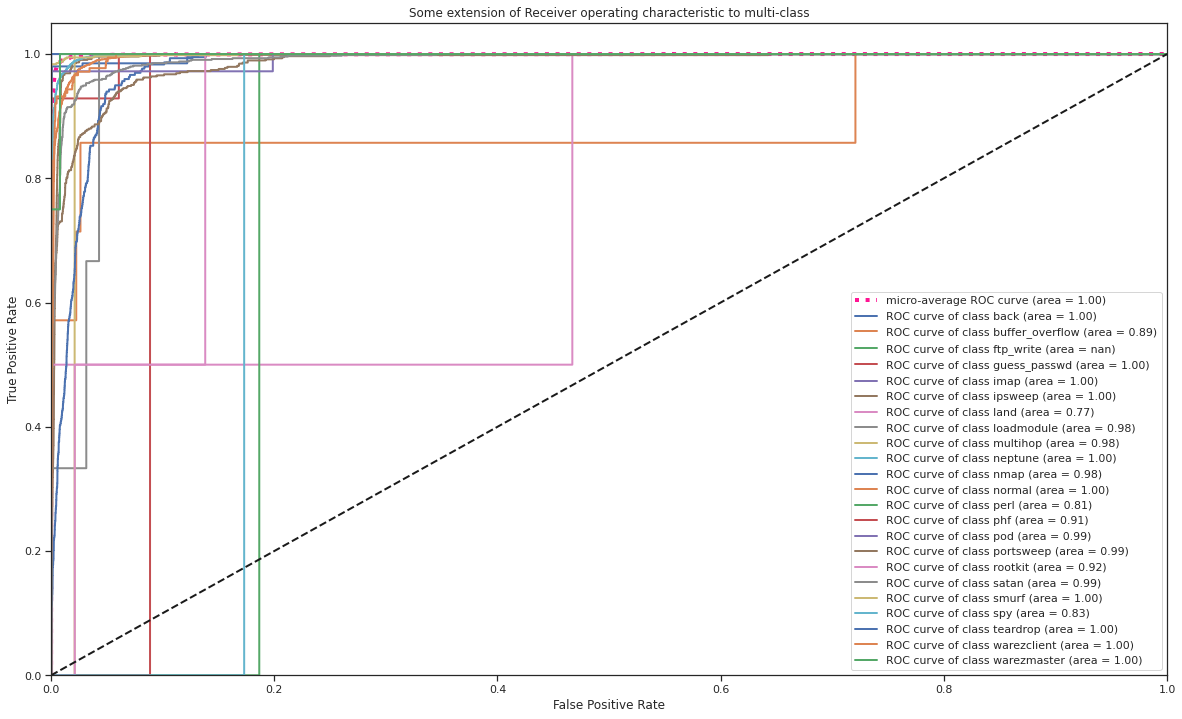
\includegraphics[width=18cm]{MLP_NSL.png}
  \caption{RoC curve of MLP on NSL-KDD Dataset}
  \label{MLP_NSL}
\end{figure}

\clearpage
\begin{figure}[h]
  \centering
  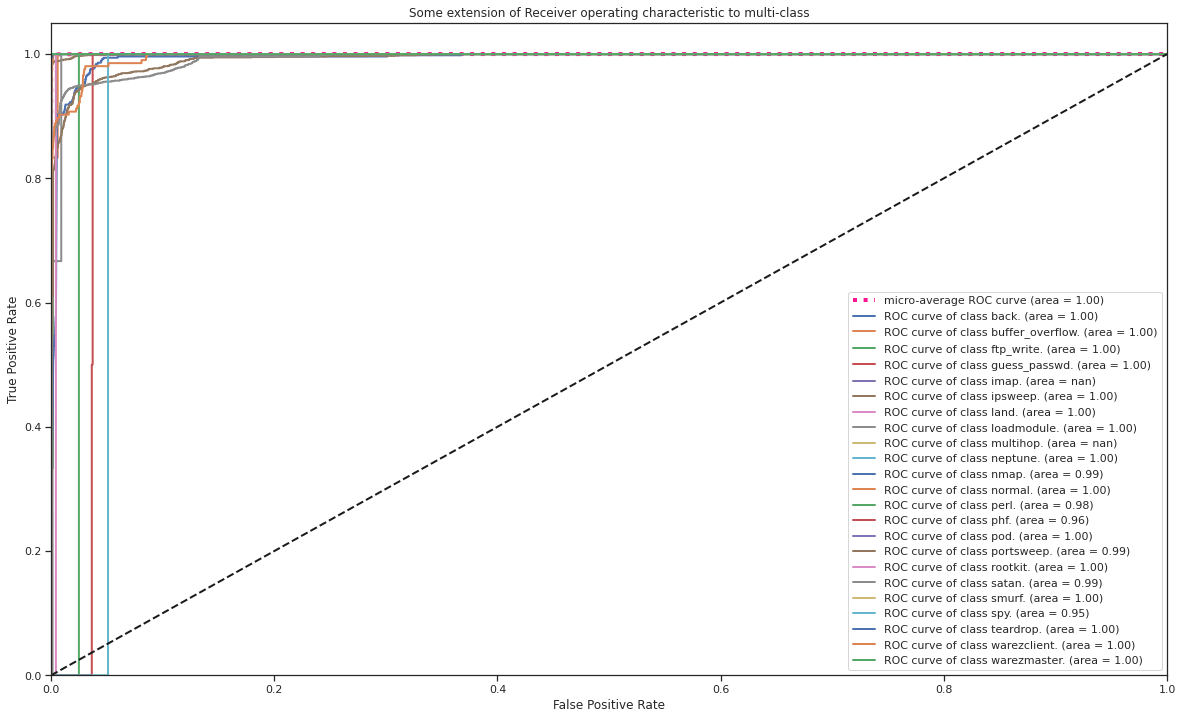
\includegraphics[width=18cm]{LSTM_KDD.png}
  \caption{RoC curve of LSTM on KDD-CUP-99 Dataset}
  \label{LSTM_KDD}
  \vspace*{\floatsep}% https://tex.stackexchange.com/q/26521/5764

  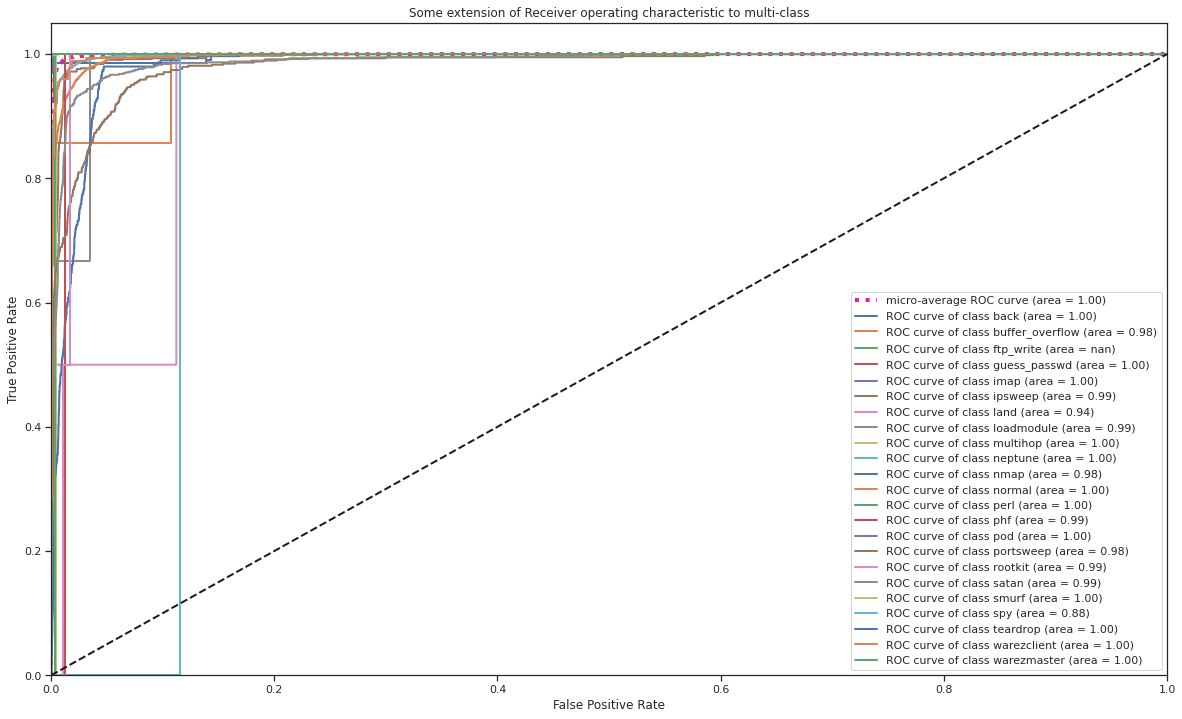
\includegraphics[width=18cm]{LSTM_NSL.png}
  \caption{RoC curve of LSTM on NSL-KDD Dataset}
  \label{LSTM_NSL}
  
\end{figure}

% \subsection{Maintaining the Integrity of the Specifications}

% The IEEEtran class file is used to format your paper and style the text. All margins, 
% column widths, line spaces, and text fonts are prescribed; please do not 
% alter them. You may note peculiarities. For example, the head margin
% measures proportionately more than is customary. This measurement 
% and others are deliberate, using specifications that anticipate your paper 
% as one part of the entire proceedings, and not as an independent document. 
% Please do not revise any of the current designations.

% \section{Prepare Your Paper Before Styling}
% Before you begin to format your paper, first write and save the content as a 
% separate text file. Complete all content and organizational editing before 
% formatting. Please note sections \ref{AA}--\ref{SCM} below for more information on 
% proofreading, spelling and grammar.

% Keep your text and graphic files separate until after the text has been 
% formatted and styled. Do not number text heads---{\LaTeX} will do that 
% for you.

% \subsection{Abbreviations and Acronyms}\label{AA}
% Define abbreviations and acronyms the first time they are used in the text, 
% even after they have been defined in the abstract. Abbreviations such as 
% IEEE, SI, MKS, CGS, ac, dc, and rms do not have to be defined. Do not use 
% abbreviations in the title or heads unless they are unavoidable.

% \subsection{Units}
% \begin{itemize}
% \item Use either SI (MKS) or CGS as primary units. (SI units are encouraged.) English units may be used as secondary units (in parentheses). An exception would be the use of English units as identifiers in trade, such as ``3.5-inch disk drive''.
% \item Avoid combining SI and CGS units, such as current in amperes and magnetic field in oersteds. This often leads to confusion because equations do not balance dimensionally. If you must use mixed units, clearly state the units for each quantity that you use in an equation.
% \item Do not mix complete spellings and abbreviations of units: ``Wb/m\textsuperscript{2}'' or ``webers per square meter'', not ``webers/m\textsuperscript{2}''. Spell out units when they appear in text: ``. . . a few henries'', not ``. . . a few H''.
% \item Use a zero before decimal points: ``0.25'', not ``.25''. Use ``cm\textsuperscript{3}'', not ``cc''.)
% \end{itemize}

% \subsection{Equations}
% Number equations consecutively. To make your 
% equations more compact, you may use the solidus (~/~), the exp function, or 
% appropriate exponents. Italicize Roman symbols for quantities and variables, 
% but not Greek symbols. Use a long dash rather than a hyphen for a minus 
% sign. Punctuate equations with commas or periods when they are part of a 
% sentence, as in:
% \begin{equation}
% a+b=\gamma\label{eq}
% \end{equation}

% Be sure that the 
% symbols in your equation have been defined before or immediately following 
% the equation. Use ``\eqref{eq}'', not ``Eq.~\eqref{eq}'' or ``equation \eqref{eq}'', except at 
% the beginning of a sentence: ``Equation \eqref{eq} is . . .''

% \subsection{\LaTeX-Specific Advice}

% Please use ``soft'' (e.g., \verb|\eqref{Eq}|) cross references instead
% of ``hard'' references (e.g., \verb|(1)|). That will make it possible
% to combine sections, add equations, or change the order of figures or
% citations without having to go through the file line by line.

% Please don't use the \verb|{eqnarray}| equation environment. Use
% \verb|{align}| or \verb|{IEEEeqnarray}| instead. The \verb|{eqnarray}|
% environment leaves unsightly spaces around relation symbols.

% Please note that the \verb|{subequations}| environment in {\LaTeX}
% will increment the main equation counter even when there are no
% equation numbers displayed. If you forget that, you might write an
% article in which the equation numbers skip from (17) to (20), causing
% the copy editors to wonder if you've discovered a new method of
% counting.

% {\BibTeX} does not work by magic. It doesn't get the bibliographic
% data from thin air but from .bib files. If you use {\BibTeX} to produce a
% bibliography you must send the .bib files. 

% {\LaTeX} can't read your mind. If you assign the same label to a
% subsubsection and a table, you might find that Table I has been cross
% referenced as Table IV-B3. 

% {\LaTeX} does not have precognitive abilities. If you put a
% \verb|\label| command before the command that updates the counter it's
% supposed to be using, the label will pick up the last counter to be
% cross referenced instead. In particular, a \verb|\label| command
% should not go before the caption of a figure or a table.

% Do not use \verb|\nonumber| inside the \verb|{array}| environment. It
% will not stop equation numbers inside \verb|{array}| (there won't be
% any anyway) and it might stop a wanted equation number in the
% surrounding equation.

% \subsection{Some Common Mistakes}\label{SCM}
% \begin{itemize}
% \item The word ``data'' is plural, not singular.
% \item The subscript for the permeability of vacuum $\mu_{0}$, and other common scientific constants, is zero with subscript formatting, not a lowercase letter ``o''.
% \item In American English, commas, semicolons, periods, question and exclamation marks are located within quotation marks only when a complete thought or name is cited, such as a title or full quotation. When quotation marks are used, instead of a bold or italic typeface, to highlight a word or phrase, punctuation should appear outside of the quotation marks. A parenthetical phrase or statement at the end of a sentence is punctuated outside of the closing parenthesis (like this). (A parenthetical sentence is punctuated within the parentheses.)
% \item A graph within a graph is an ``inset'', not an ``insert''. The word alternatively is preferred to the word ``alternately'' (unless you really mean something that alternates).
% \item Do not use the word ``essentially'' to mean ``approximately'' or ``effectively''.
% \item In your paper title, if the words ``that uses'' can accurately replace the word ``using'', capitalize the ``u''; if not, keep using lower-cased.
% \item Be aware of the different meanings of the homophones ``affect'' and ``effect'', ``complement'' and ``compliment'', ``discreet'' and ``discrete'', ``principal'' and ``principle''.
% \item Do not confuse ``imply'' and ``infer''.
% \item The prefix ``non'' is not a word; it should be joined to the word it modifies, usually without a hyphen.
% \item There is no period after the ``et'' in the Latin abbreviation ``et al.''.
% \item The abbreviation ``i.e.'' means ``that is'', and the abbreviation ``e.g.'' means ``for example''.
% \end{itemize}
% An excellent style manual for science writers is \cite{b7}.

% \subsection{Authors and Affiliations}
% \textbf{The class file is designed for, but not limited to, six authors.} A 
% minimum of one author is required for all conference articles. Author names 
% should be listed starting from left to right and then moving down to the 
% next line. This is the author sequence that will be used in future citations 
% and by indexing services. Names should not be listed in columns nor group by 
% affiliation. Please keep your affiliations as succinct as possible (for 
% example, do not differentiate among departments of the same organization).

% \subsection{Identify the Headings}
% Headings, or heads, are organizational devices that guide the reader through 
% your paper. There are two types: component heads and text heads.

% Component heads identify the different components of your paper and are not 
% topically subordinate to each other. Examples include Acknowledgments and 
% References and, for these, the correct style to use is ``Heading 5''. Use 
% ``figure caption'' for your Figure captions, and ``table head'' for your 
% table title. Run-in heads, such as ``Abstract'', will require you to apply a 
% style (in this case, italic) in addition to the style provided by the drop 
% down menu to differentiate the head from the text.

% Text heads organize the topics on a relational, hierarchical basis. For 
% example, the paper title is the primary text head because all subsequent 
% material relates and elaborates on this one topic. If there are two or more 
% sub-topics, the next level head (uppercase Roman numerals) should be used 
% and, conversely, if there are not at least two sub-topics, then no subheads 
% should be introduced.

% \subsection{Figures and Tables}
% \paragraph{Positioning Figures and Tables} Place figures and tables at the top and 
% bottom of columns. Avoid placing them in the middle of columns. Large 
% figures and tables may span across both columns. Figure captions should be 
% below the figures; table heads should appear above the tables. Insert 
% figures and tables after they are cited in the text. Use the abbreviation 
% ``Fig.~\ref{fig}'', even at the beginning of a sentence.

% \begin{table}[htbp]
% \caption{Table Type Styles}
% \begin{center}
% \begin{tabular}{|c|c|c|c|}
% \hline
% \textbf{Table}&\multicolumn{3}{|c|}{\textbf{Table Column Head}} \\
% \cline{2-4} 
% \textbf{Head} & \textbf{\textit{Table column subhead}}& \textbf{\textit{Subhead}}& \textbf{\textit{Subhead}} \\
% \hline
% copy& More table copy$^{\mathrm{a}}$& &  \\
% \hline
% \multicolumn{4}{l}{$^{\mathrm{a}}$Sample of a Table footnote.}
% \end{tabular}
% \label{tab1}
% \end{center}
% \end{table}

% \begin{figure}[htbp]
% \centerline{\includegraphics{fig1.png}}
% \caption{Example of a figure caption.}
% \label{fig}
% \end{figure}

% Figure Labels: Use 8 point Times New Roman for Figure labels. Use words 
% rather than symbols or abbreviations when writing Figure axis labels to 
% avoid confusing the reader. As an example, write the quantity 
% ``Magnetization'', or ``Magnetization, M'', not just ``M''. If including 
% units in the label, present them within parentheses. Do not label axes only 
% with units. In the example, write ``Magnetization (A/m)'' or ``Magnetization 
% \{A[m(1)]\}'', not just ``A/m''. Do not label axes with a ratio of 
% quantities and units. For example, write ``Temperature (K)'', not 
% ``Temperature/K''.

% \section*{Acknowledgment}

% The preferred spelling of the word ``acknowledgment'' in America is without 
% an ``e'' after the ``g''. Avoid the stilted expression ``one of us (R. B. 
% G.) thanks $\ldots$''. Instead, try ``R. B. G. thanks$\ldots$''. Put sponsor 
% acknowledgments in the unnumbered footnote on the first page.

% \section*{References}

% Please number citations consecutively within brackets \cite{b1}. The 
% sentence punctuation follows the bracket \cite{b2}. Refer simply to the reference 
% number, as in \cite{b3}---do not use ``Ref. \cite{b3}'' or ``reference \cite{b3}'' except at 
% the beginning of a sentence: ``Reference \cite{b3} was the first $\ldots$''

% Number footnotes separately in superscripts. Place the actual footnote at 
% the bottom of the column in which it was cited. Do not put footnotes in the 
% abstract or reference list. Use letters for table footnotes.

% Unless there are six authors or more give all authors' names; do not use 
% ``et al.''. Papers that have not been published, even if they have been 
% submitted for publication, should be cited as ``unpublished'' \cite{b4}. Papers 
% that have been accepted for publication should be cited as ``in press'' \cite{b5}. 
% Capitalize only the first word in a paper title, except for proper nouns and 
% element symbols.

% For papers published in translation journals, please give the English 
% citation first, followed by the original foreign-language citation \cite{b6}.

\clearpage
\bibliographystyle{unsrt}
\bibliography{bib.bib}

\vspace{12pt}
% \color{red}
% IEEE conference templates contain guidance text for composing and formatting conference papers. Please ensure that all template text is removed from your conference paper prior to submission to the conference. Failure to remove the template text from your paper may result in your paper not being published.

\end{document}
